% Created 2019-09-22 Sun 16:10
% Intended LaTeX compiler: pdflatex
\documentclass[10pt,t]{beamer}
\usepackage[utf8]{inputenc}
\usepackage[T1]{fontenc}
\usepackage{graphicx}
\usepackage{grffile}
\usepackage{longtable}
\usepackage{wrapfig}
\usepackage{rotating}
\usepackage{amsmath}
\usepackage{textcomp}
\usepackage{amssymb}
\usepackage{capt-of}
\usepackage{hyperref}
\usetheme{default}
\author{L. Larrabee Strow}
\date{\today}
\title{\large AIRS Calibration for Climate Trend Studies: Status and Future}
\subtitle{\footnotesize{AIRS Science Team Meeting}}
\date{\vspace{0.1in}\footnotesize{September 25, 201\vfill}}
\author{L. Larrabee Strow\inst{1,2}}
\institute[UMBC]{\inst{1} UMBC Physics Dept. \and \inst{2}UMBC JCET}
\input beamer_setup
\usetheme{metropolis}
\metroset{titleformat title=allcaps}
\renewcommand{\UrlFont}{\small\tt}
\renewcommand*{\UrlFont}{\footnotesize}
\tolerance=1000
\RequirePackage{fancyvrb}
\DefineVerbatimEnvironment{verbatim}{Verbatim}{fontsize=\footnotesize}
\begin{document}

\maketitle
\addtobeamertemplate{block begin}{
  \setlength{\parsep}{0pt}
  \setlength{\topsep}{3pt plus 2pt minus 2.5pt}
  \setlength{\itemsep}{0pt plus 0pt minus 2pt}
  \setlength{\partopsep}{2pt}
}


\begin{frame}[label={sec:org123901d},shrink=30]{Calibration Requirements for Climate Science}
\vspace{-0.1in}
\begin{large}
\begin{itemize}
\item AIRS 17+ year record long enough to address key climate questions
\item Stability of radiometric calibration is key
\item AIRS sensitivity to \cd, SST, etc allows stringent tests of stability
\end{itemize}
\end{large}
\vspace{-0.2in}
\begin{columns}
\begin{column}{0.55\columnwidth}
\begin{block}{Climate Science Questions}
\vspace{0.05in}
\emph{All require min \textasciitilde{}0.1K/decade stability}
\vspace{-0.05in}
\begin{itemize}
\item Global Trending: T(z), \water(z), T\textsubscript{surf}
\item Water vapor feedback (Does relative humidity vary)
\item Cloud feedback
\item Trends in PBL cloud occurance
\item OLR anomalies separated by cause: T/\water/cloud/surface, etc.
\end{itemize}
\end{block}
\end{column}

\begin{column}{0.55\columnwidth}
\begin{block}{Hyperspectral IR Advantages}
\begin{itemize}
\item AIRS senses both climate forcings, and responses
\item Clean separation of tropospheric vs stratospheric temperature trends (unlike microwave)
\item Multiple long-term overlapping missions (AIRS, CrIS, IASI)
\item AIRS, CrIS, IASI aleady agree to \textasciitilde{}0.1-0.3K and can be merged to 0.03K or better.
\end{itemize}
\end{block}
\end{column}
\end{columns}



\vspace{0.2in}
\begin{large}
Significant AIRS calibration drifts have \alert{already} resulted publication of in-accurate data that were publized by NASA/GSFC and the media (Washington Post, Scientific American).  \emph{This talk suggests how to make AIRS an accurate instrument for climate science.}
\end{large}
\end{frame}

\begin{frame}[label={sec:org83a03ca},shrink=20]{Weather versus Climate Research}
\begin{block}{Weather Applications}
\begin{itemize}
\item AIRS original focus was for NWP
\item Both 1Dvar retrievals and data assimilation \emph{require} bias removal
\begin{itemize}
\item NWP: biases due to the instrument, RTA, model
\item Retrievals: biases due to the instrument and RTA
\item Bias removal is generally in the \textasciitilde{}0.1-0.3K range
\end{itemize}
\item Radiometric accuracy is important
\begin{itemize}
\item But, below the nominal \textasciitilde{}0.3K range we cannot differentiate instrument vs RTA errors.
\item Spectroscopy errors are at the 1-2\% level, or 0.1-0.3K
\end{itemize}
\end{itemize}
\end{block}
\begin{block}{Climate Applications}
\begin{itemize}
\item Anomalies are the main language of climate observations
\item Although energy budget and fluxes are important, AIRS is not a major contributor
\item For AIRS, radiometric stability is most fundamental calibration requirement
\end{itemize}

Hyperspectral IR instrument stability appears to be 1-2 orders of magnitude better than absolute accuracy.  This is where we can shine, especially with a 17+ year record.
\end{block}
\end{frame}

\begin{frame}[label={sec:org24ce98f},shrink=5]{Climate Product Characteristics}
\begin{block}{Uncertainty Estimates}
\begin{itemize}
\item If we provide something unique, validation will be difficult
\item Internal product uncertainty estimates will be far more important than for weather applciations
\item Establishing uncertainites for products is a NASA ROSES requirement!
\end{itemize}
\end{block}

\begin{block}{Reproducibility}
\begin{itemize}
\item Reproducibiity of results is becoming increasingly important
\item Difficlt to achieve with our Level 2 approach
\item For climate simpler algorithms with reproducible results would enhance our impact on the broader community
\end{itemize}

There is a long history of controversies in climate measurements (esp. microwave temperature trends).  AIRS derived results will be heavily scrutinized, we need to be prepared for that to retain trust.
\end{block}
\end{frame}

\begin{frame}[label={sec:orgf4ace31}]{AIRS Stability Calibration: An Approach}
\begin{itemize}
\item External standards needed to establish stability
\item \cd and possibly \nitrous and \methane can provide those standards
\begin{itemize}
\item \cd is well mixed (on long time scales) and extremely well known
\item Establish AIRS stability by retrieving \cd anomalies (vs time)
\end{itemize}
\item SST is the other well established climate record
\begin{itemize}
\item Similarly, use retrieved SST anomalies to test AIRS stability
\end{itemize}
\item Land surface temperatures are another possibility, although less reliable than SST but of great interest and heavily studied.
\end{itemize}

Essentially you need to perform climate-level retrievals to test the capabilities of your instrument.  

A \emph{key} requirement is the need to reprocess the \emph{full record} many times.  NOT possible with Level 2 approach!  Need fast alternatives that may also address issues of reproducibility.
\end{frame}

\begin{frame}[label={sec:org35e37f9}]{Characteristics of AIRs Long-Term Radiance Trends}
\begin{itemize}
\item 1\% random subset
\end{itemize}
\end{frame}
\begin{frame}[label={sec:org4503062}]{AIRS Global 16-Year B(T) Trend}
\vspace{-0.35in}

\begin{columns}
\begin{column}{0.55\columnwidth}
\begin{block}{\footnotesize All channels (inc. fill)}
\vspace{-0.1in}
\begin{center}
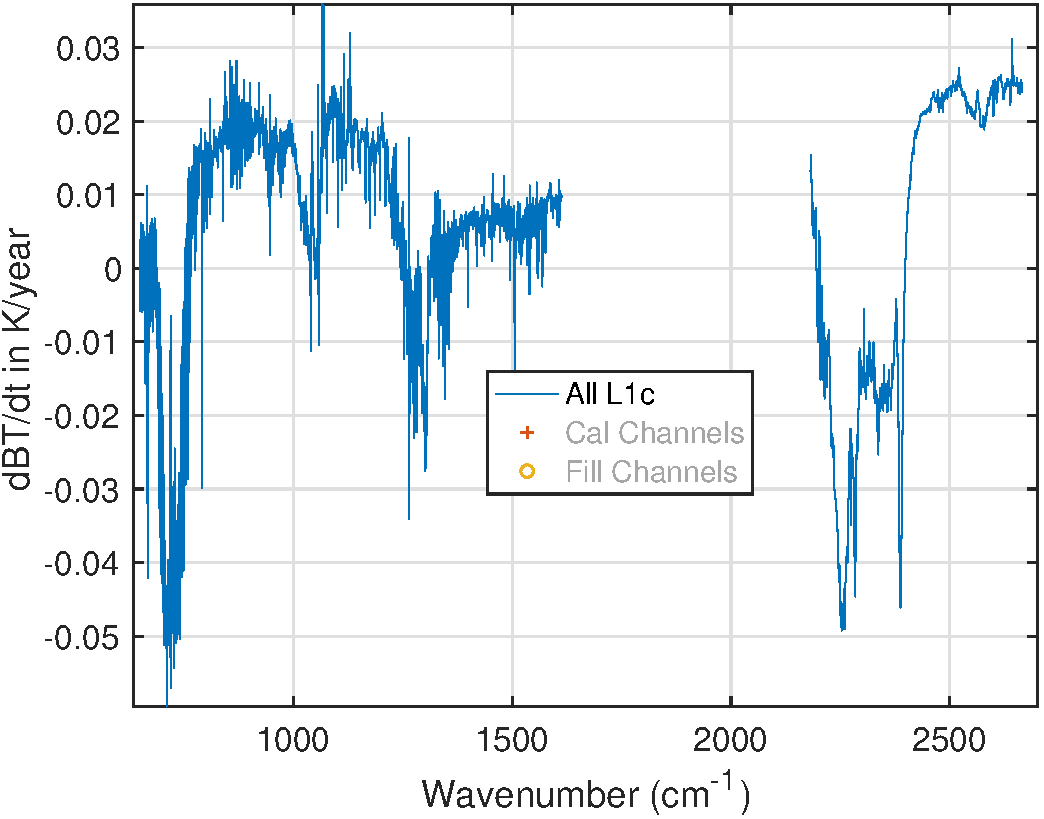
\includegraphics[width=0.85\linewidth]{./Figs/Pdf/rand_global_trend_l1c_overview.pdf}
\end{center}
\end{block}
\end{column}


\begin{column}{0.55\columnwidth}
\begin{block}{\footnotesize Fill channels marked}
\vspace{-0.1in}
\begin{center}
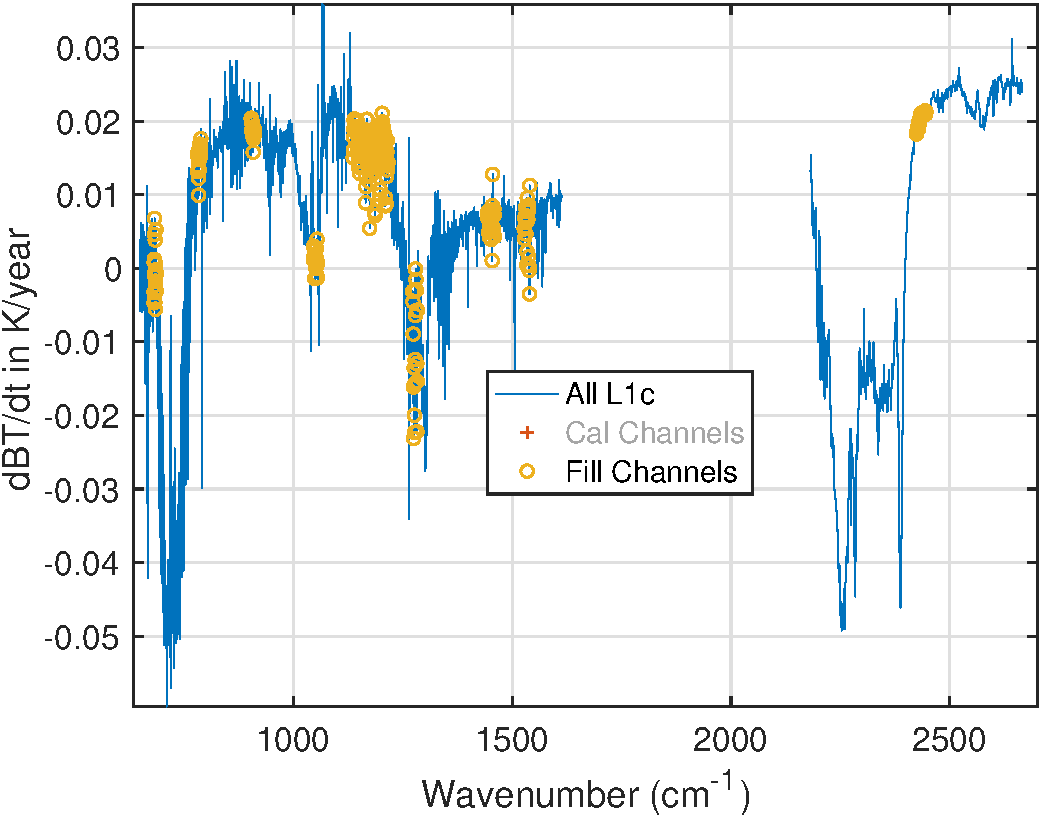
\includegraphics[width=0.85\linewidth]{./Figs/Pdf/rand_global_trend_l1c_overview_fill_marked.pdf}
\end{center}
\end{block}
\end{column}
\end{columns}


\vspace{-0.25in}

\begin{columns}
\begin{column}{0.55\columnwidth}
\begin{block}{\footnotesize Calibration channels}
\vspace{-0.1in}
\begin{center}
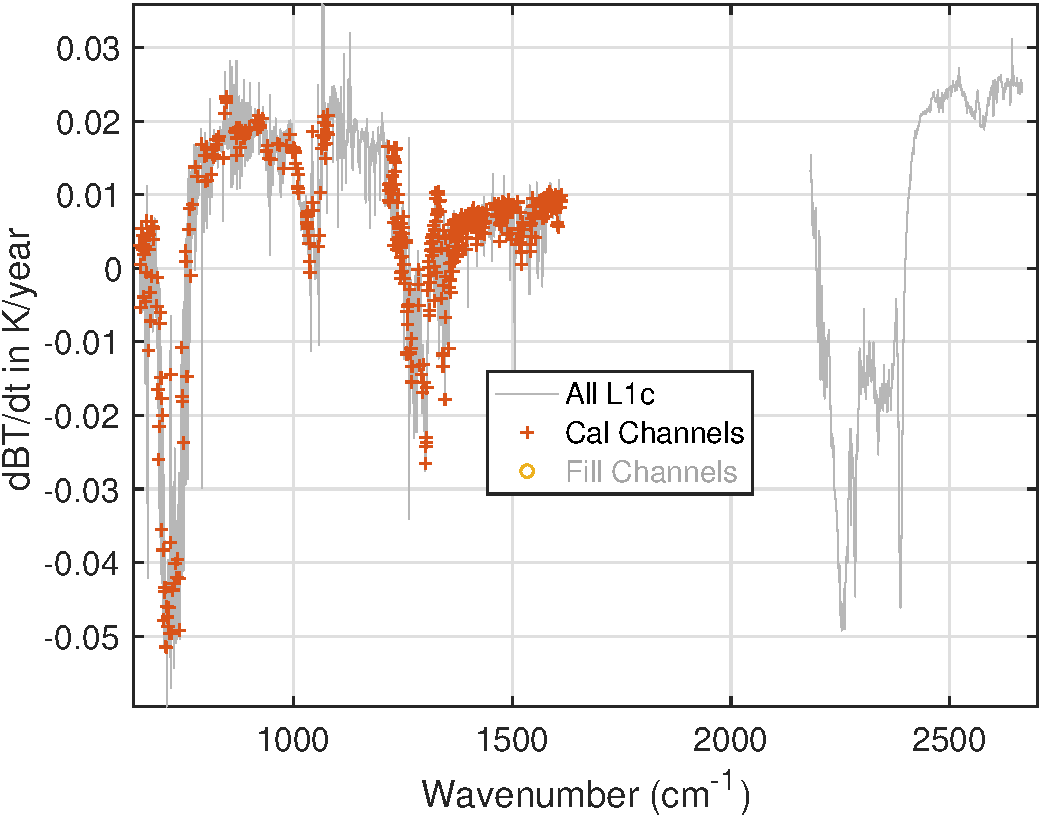
\includegraphics[width=0.75\linewidth]{./Figs/Pdf/rand_global_trend_l1c_overview_calfit_marked.pdf}
\end{center}
\end{block}
\end{column}


\begin{column}{0.55\columnwidth}
\begin{block}{\footnotesize}
\begin{footnotesize}
Channels used for calibration testing marked.\\
\vspace{0.05in}
These channels have no A/B state changes, good S/N, small drift\\
\vspace{0.05in}
Note sparsity of \cd channels in tropospheric sounding region\\
\end{footnotesize}
\end{block}
\end{column}
\end{columns}
\end{frame}

\begin{frame}[label={sec:orga4bf877}]{\cd and \methane Trends Removed, Fitted Chans Only}
\vspace{-0.3in}
\begin{columns}
\begin{column}{0.55\columnwidth}
\begin{block}{\footnotesize AIRS + ERA}
\vspace{-0.1in}
\begin{center}
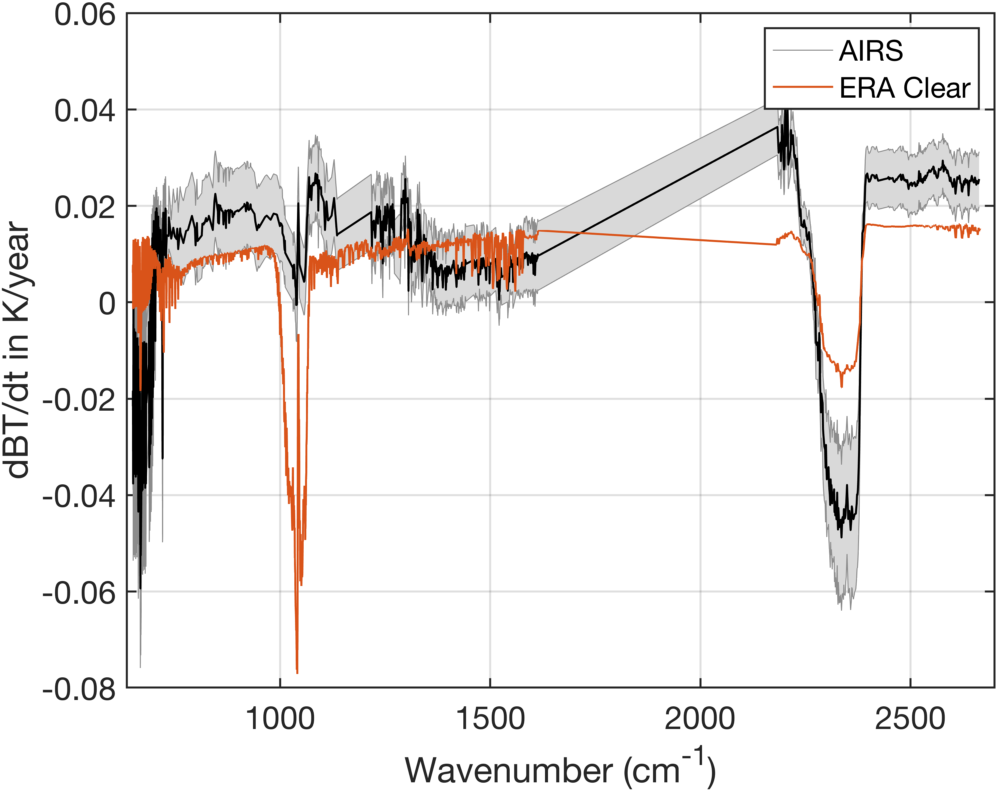
\includegraphics[width=\linewidth]{./Figs/Png/rand_global_trend_l1c_vs_era_clr_only_fit_chans.png}
\end{center}
\end{block}
\end{column}

\begin{column}{0.55\columnwidth}
\begin{block}{\footnotesize AIRS w/ 0.02K dT, RH constant}
\vspace{-0.1in}
\begin{center}
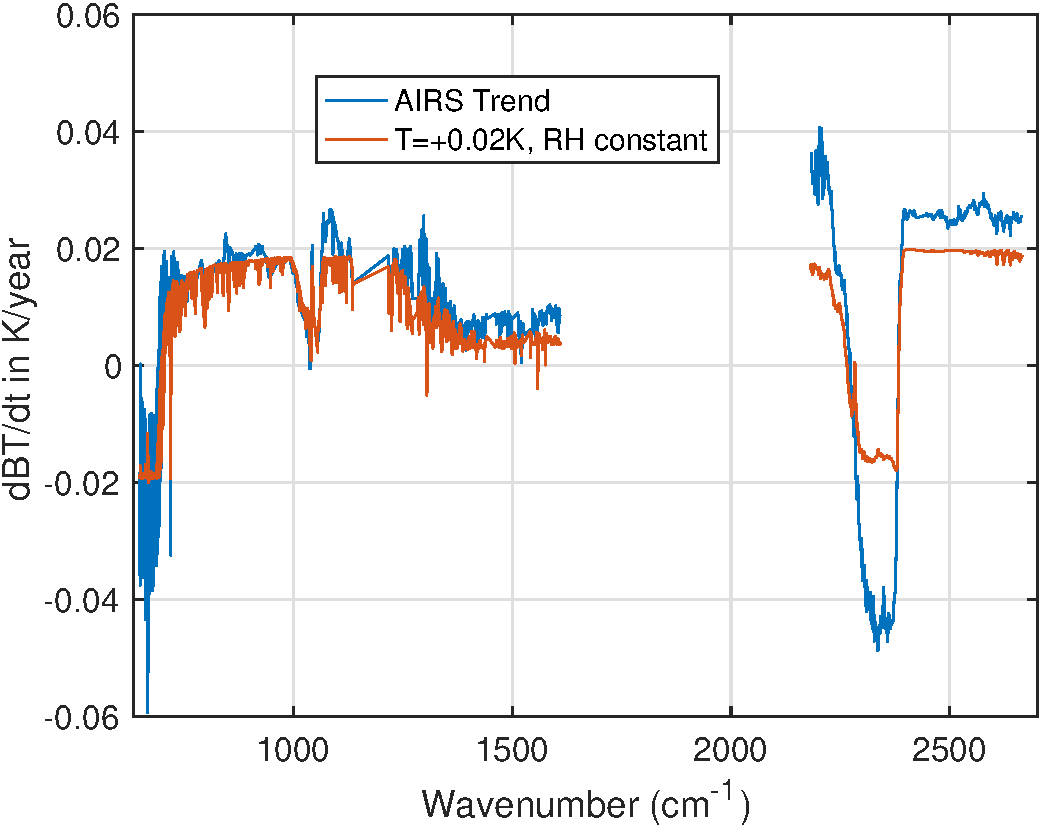
\includegraphics[width=\linewidth]{./Figs/Pdf/dbt_constantRH_dsurf_dtrop=0.02k_dstrat=m0.02k_withAIRS.pdf}
\end{center}
\end{block}
\end{column}
\end{columns}

\begin{small}
\begin{itemize}
\item Uncertainty (gray) is geophysical (Std over latitutde).
\item RHS: Trop T(z) + 0.02K, Strat T(z) - 0.02K
\item \water trend is close to constant RH. (Varies with latitude).
\item Could suggest RH is a bit lower over time??
\item Shortwave appears to have a positive drift
\end{itemize}
\end{small}
\end{frame}

\begin{frame}[label={sec:orgdef18f4}]{Retrieval of \cd, \nitrous, \methane Anomalies}
\begin{itemize}
\item oem approach
\item data set
\item kcarta vs sarta
\item true noise, averaged over \textasciitilde{}600 pts/16 days per 1/40 lat bins.
\item 2ppm \cd a-priori covariance, with 2ppm slope a=prori, 5 ppm covariance almost as good
\item jacobian (kernel) profiles from ERA, but we could fit for them,
\item iterate: first remove jumps due to know events in fitting channels
\item then evaluate channels not fitted, and include if warranted
\item possible  BB is stable
\item relative channel errors are likely due to small thermal changes changing view of cold space, etc.  a/b often different
\end{itemize}
\end{frame}
\begin{frame}[label={sec:orga1eeb73}]{\cd Anomaly Fit for MLO Latitude}
\vspace{-0.3in}
\begin{columns}
\begin{column}{0.55\columnwidth}
\begin{block}{\footnotesize Fitting Trick}
\begin{center}
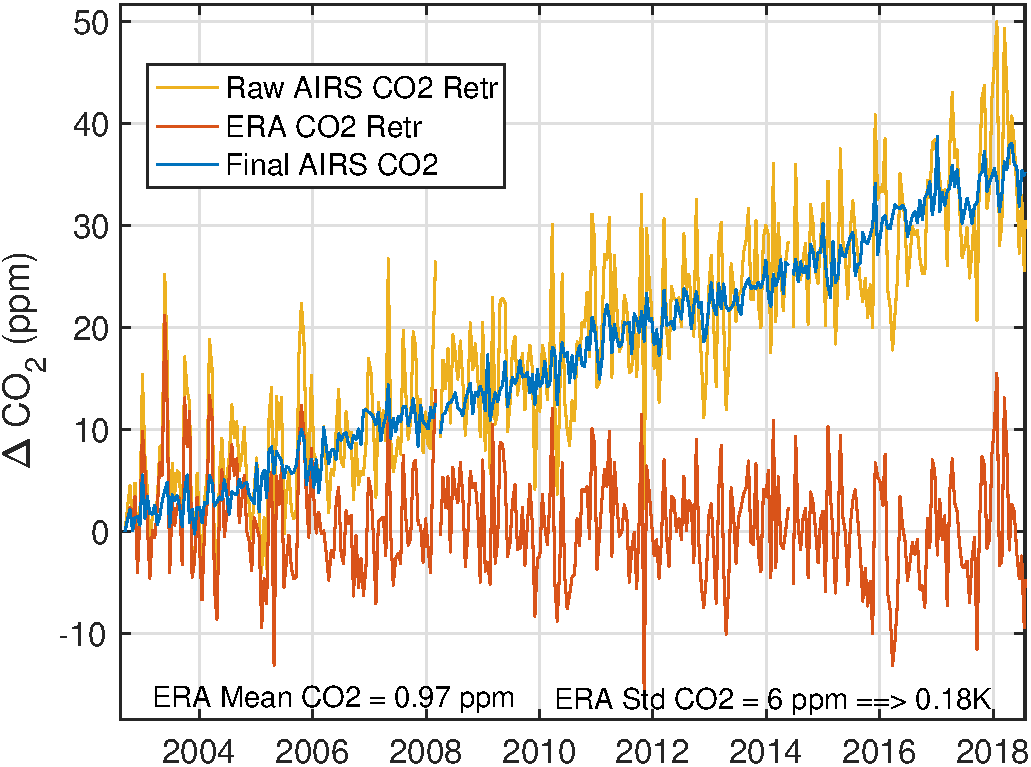
\includegraphics[width=\linewidth]{./Figs/Pdf/raw_co2_vs_era_co2_example_lati28_mlo_lat.pdf}
\end{center}
\end{block}
\end{column}

\begin{column}{0.55\columnwidth}
\begin{block}{\footnotesize Fitted \cd Anomalies}
\begin{center}
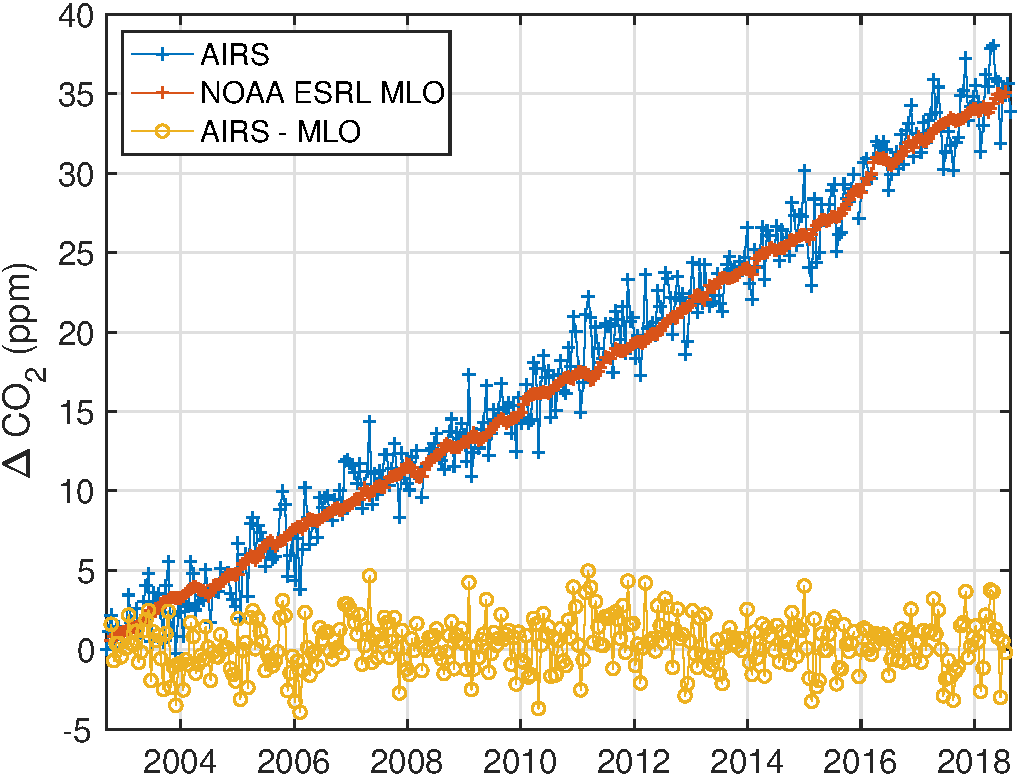
\includegraphics[width=\linewidth]{./Figs/Pdf/co2_airs_vs_mlo.pdf}
\end{center}
\end{block}
\end{column}
\end{columns}

\begin{footnotesize}
\begin{itemize}
\item ERA simulations done per footprint
\item Fit ERA simulation for \cd
\item Removes co-linearity? and lowers "noise"
\end{itemize}
\end{footnotesize}
\end{frame}

\begin{frame}[label={sec:org028daca}]{\cd Anomaly Converted to B(T) Trends}
\begin{center}
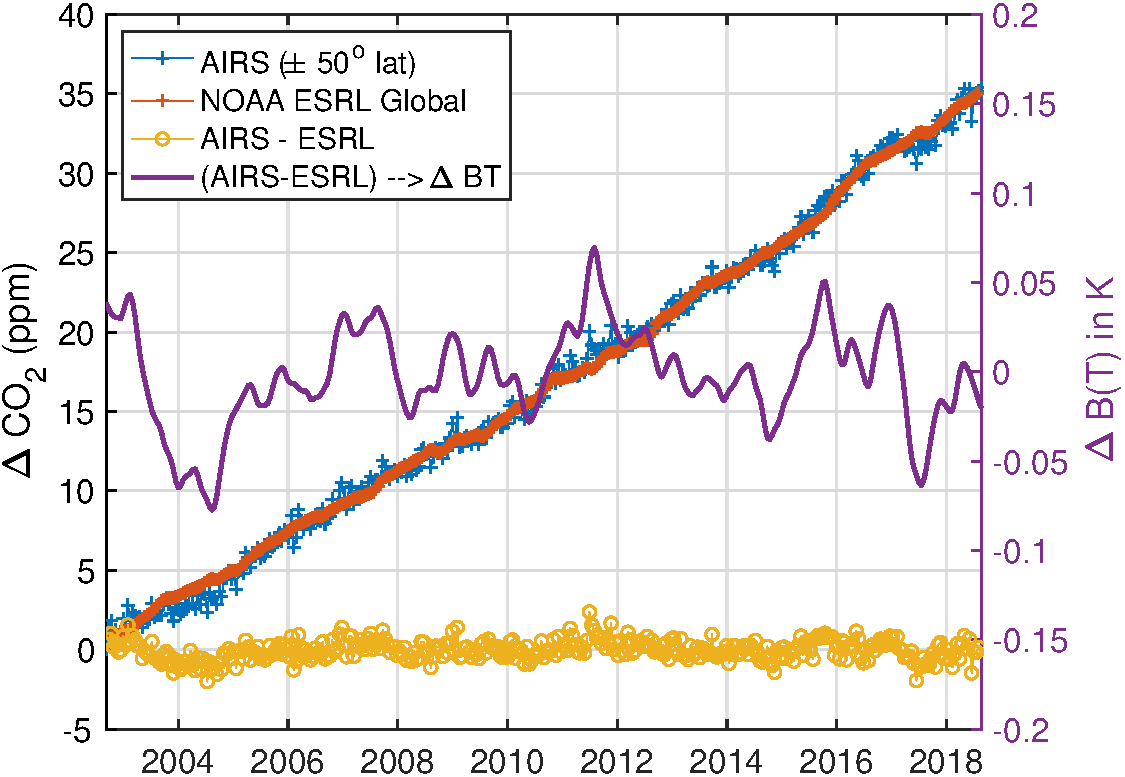
\includegraphics[width=0.7\linewidth]{./Figs/Pdf/co2_airs_vs_esrl_global_with_dbt.pdf}
\end{center}
\end{frame}

\begin{frame}[label={sec:orgf2793ca}]{Other \cd Diagnostics}
\vspace{-0.35in}
\begin{columns}
\begin{column}{0.5\columnwidth}
\begin{block}{\footnotesize Growth Rates}
\vspace{-0.1in}
\begin{center}
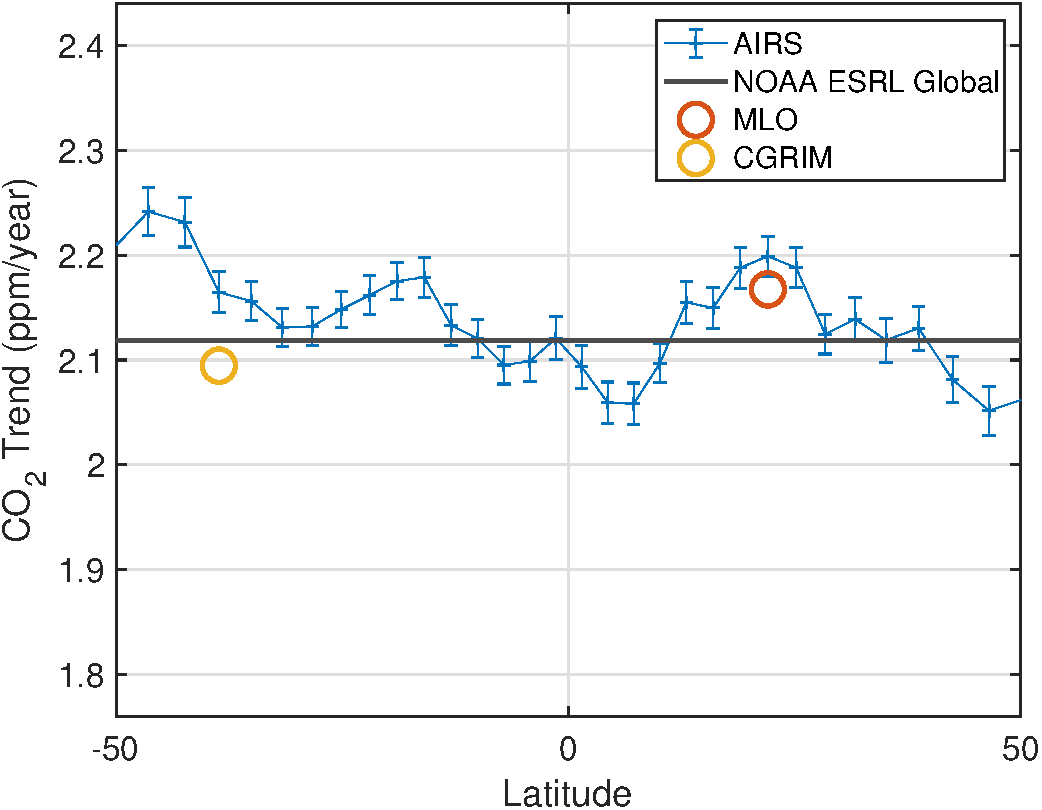
\includegraphics[width=0.9\linewidth]{./Figs/Pdf/co2_growth_vs_lat.pdf}
\end{center}
\end{block}
\end{column}

\begin{column}{0.5\columnwidth}
\begin{block}{\footnotesize Growth Rate Anomaly}
\vspace{-0.1in}
\begin{center}
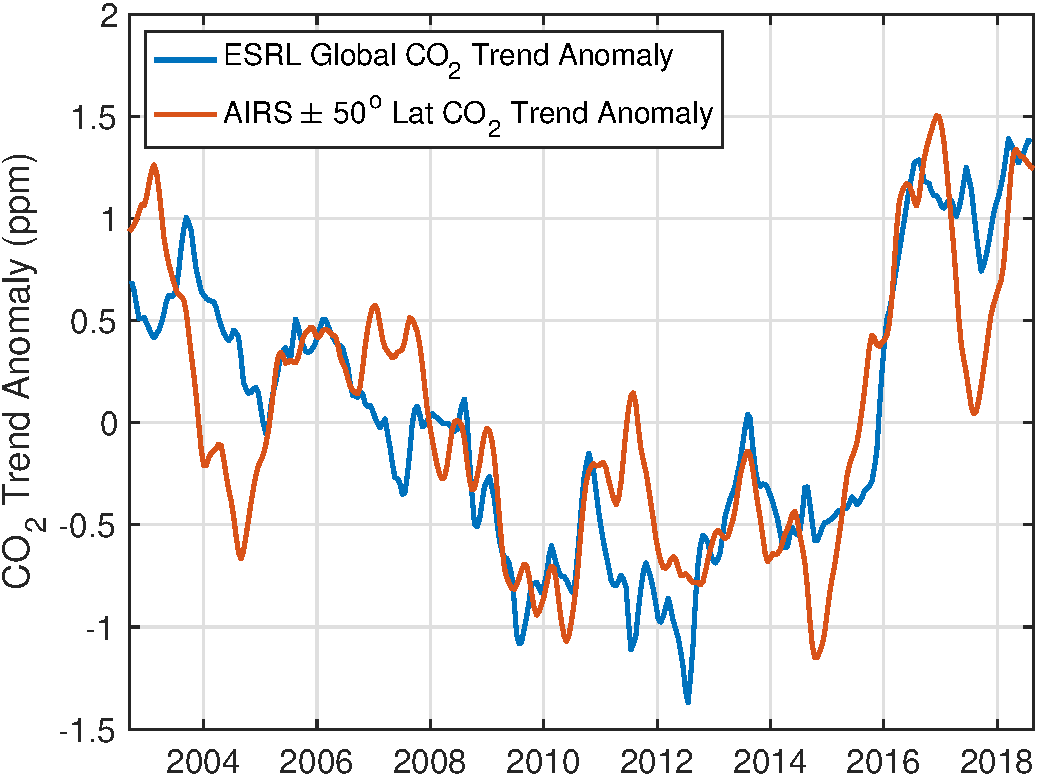
\includegraphics[width=0.9\linewidth]{./Figs/Pdf/co2_airs_vs_esrl_global_growth_anom.pdf}
\end{center}
\end{block}
\end{column}
\end{columns}

\vspace{-0.2in}

\begin{columns}
\begin{column}{0.5\columnwidth}
\begin{block}{\footnotesize Zonal Anomalies}
\vspace{-0.1in}
\begin{center}
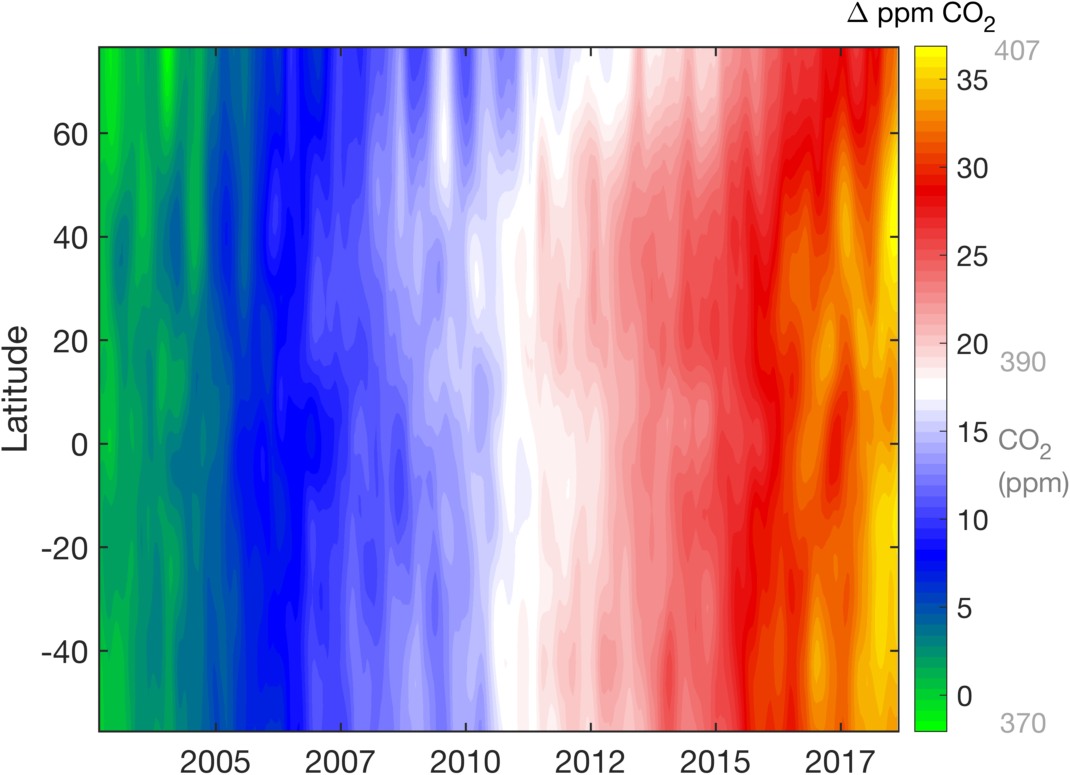
\includegraphics[width=0.9\linewidth]{./Figs/Png/co2_anom_image_lat_vs_time.png}
\end{center}
\end{block}
\end{column}

\begin{column}{0.5\columnwidth}
\begin{block}{}
\footnotesize Growth rate anomaly accuracy very encouraging.
\end{block}
\end{column}
\end{columns}
\end{frame}

\begin{frame}[label={sec:orgbc41163}]{\nitrous Retrieved Anomalies}
\begin{center}
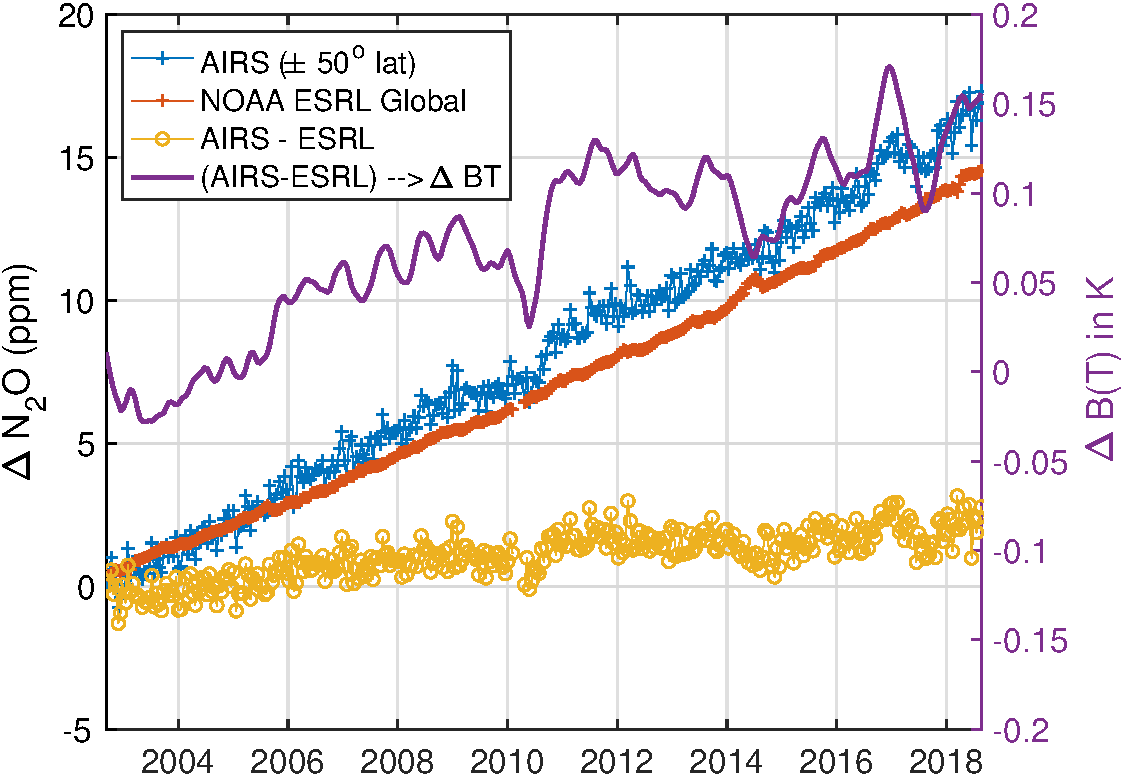
\includegraphics[width=0.7\linewidth]{./Figs/Pdf/n2o_airs_vs_esrl_global_with_dbt.pdf}
\end{center}

\begin{footnotesize}
\begin{itemize}
\item This is what we are after
\item Something a little before 2006?
\item A jump due to the Jan. 2010 shutdown
\item Stable otherwise
\item Look at residuals of fits to understand guilty channels
\end{itemize}
\end{footnotesize}
\end{frame}

\begin{frame}[label={sec:org4afcc39}]{\methane Retrieved Anomalies}
\begin{center}
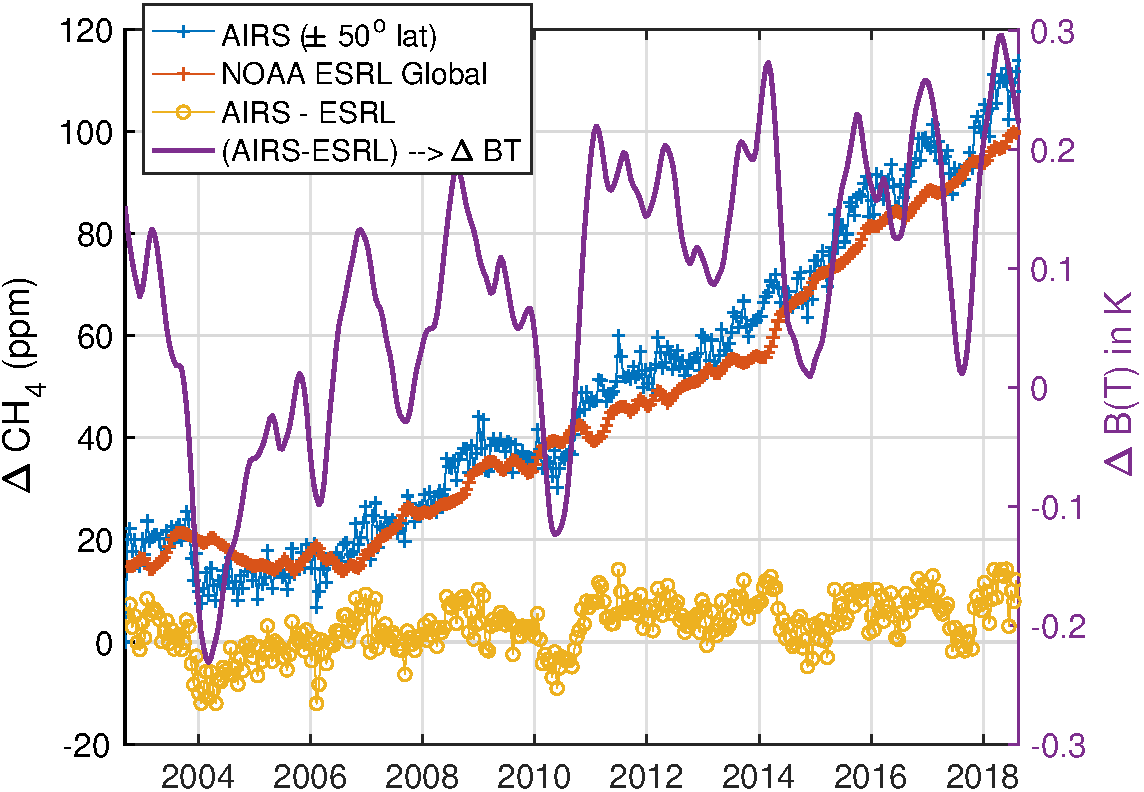
\includegraphics[width=0.7\linewidth]{./Figs/Pdf/ch4_airs_vs_esrl_global_with_dbt.pdf}
\end{center}

\begin{footnotesize}
\begin{itemize}
\item Is \methane well mixed enough for this analysis?
\item Clearly an offset in Jan 2010 but it recovered (seen in spectral!)
\item Clear Nov. 2003 B(T) shift
\end{itemize}
\end{footnotesize}
\end{frame}

\begin{frame}[label={sec:org7b9eba2}]{\methane Growth Rate Anomalies}
\begin{center}
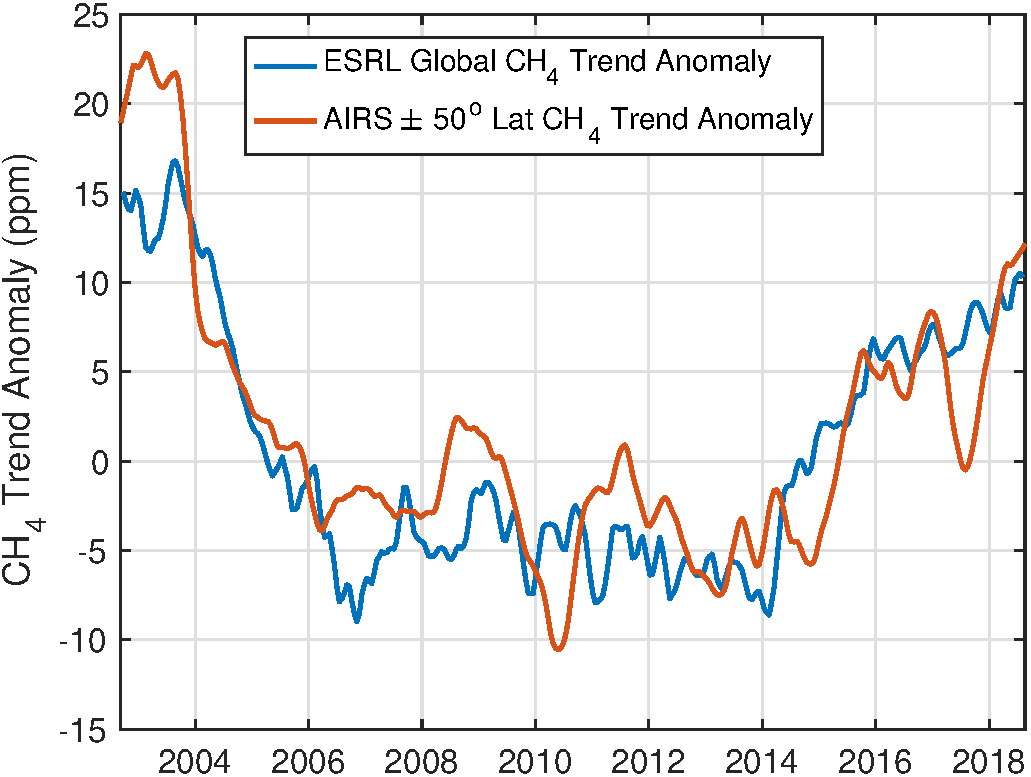
\includegraphics[width=0.7\linewidth]{./Figs/Pdf/ch4_airs_vs_esrl_global_growth_anom.pdf}
\end{center}

\begin{footnotesize}
\begin{itemize}
\item Very nice agreement with NOAA ESRL in-situ
\item Shows drop-off in global \methane growth early in mission
\item Then increasing growth starting in 2014
\end{itemize}
\end{footnotesize}
\end{frame}

\begin{frame}[label={sec:orgd95e21f}]{Unlike Retrievals We'd Like to Examine Many Channels}
\vspace{-0.3in}

\begin{columns}
\begin{column}{0.55\columnwidth}
\begin{block}{\footnotesize IASI: 11-Year Trend}
\vspace{-0.1in}
\begin{center}
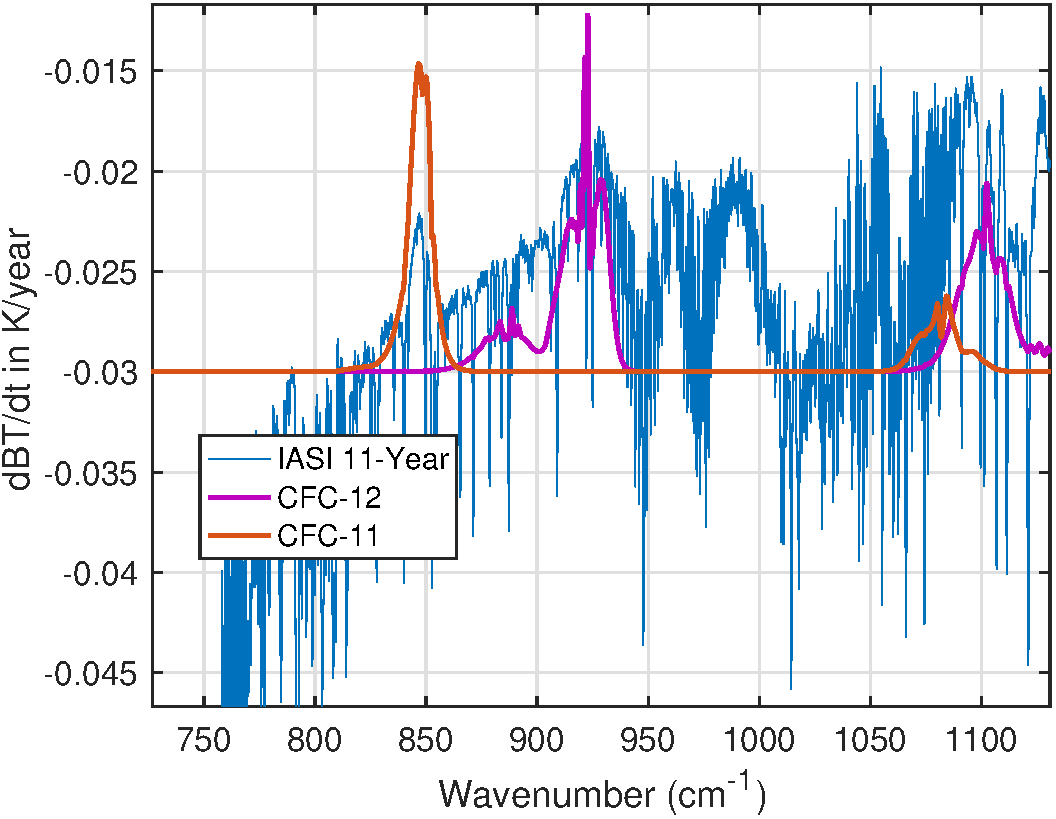
\includegraphics[width=0.75\linewidth]{./Figs/Pdf/iasi_cfc_signatures.pdf}
\end{center}
\end{block}
\end{column}

\begin{column}{0.55\columnwidth}
\begin{block}{\footnotesize}
\begin{footnotesize}
That means taking the CFC 11 and 12 into account.\\
\vspace{0.05in}
Maybe 3 strong CFC 11 channels?\\
\vspace{0.05in}
Maybe 3-5 strong CFC 12 channels?\\
\vspace{0.05in}
But, need to remove effects in wings
\end{footnotesize}
\end{block}
\end{column}
\end{columns}

\vspace{-0.25in}

\begin{columns}
\begin{column}{0.55\columnwidth}
\begin{block}{\footnotesize IASI Trend Zoom}
\vspace{-0.1in}
\begin{center}
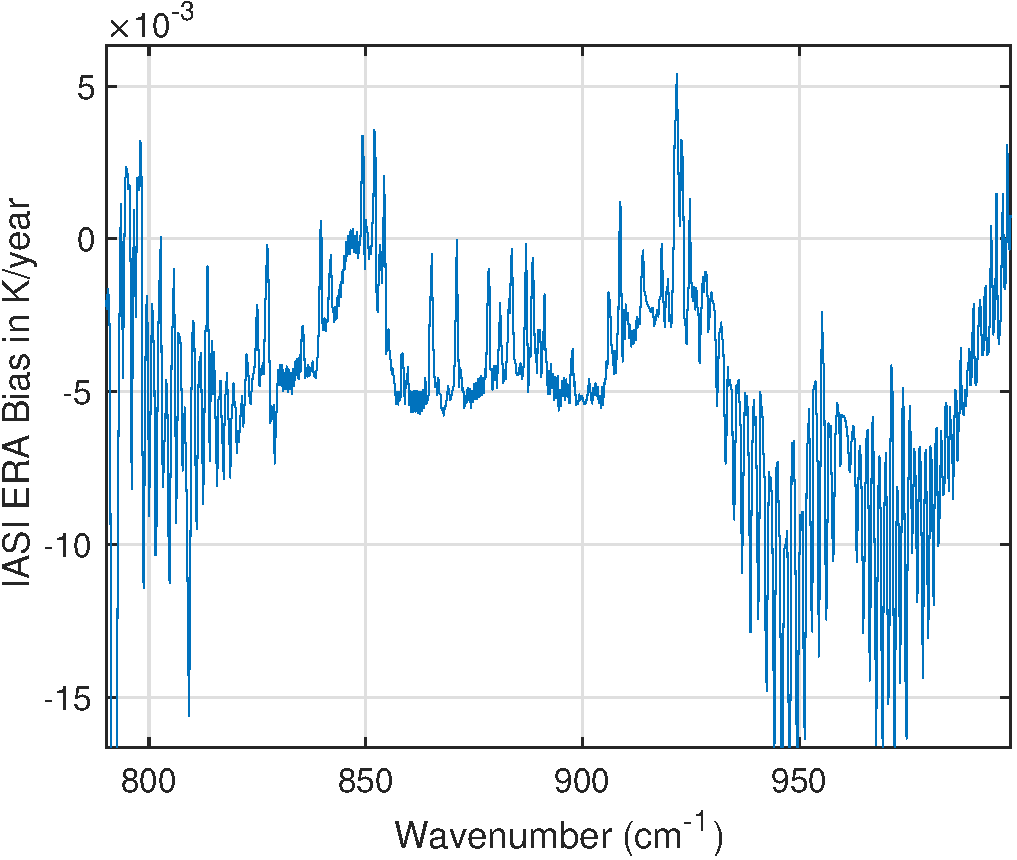
\includegraphics[width=0.75\linewidth]{./Figs/Pdf/iasi_cfc_bias.pdf}
\end{center}
\end{block}
\end{column}

\begin{column}{0.55\columnwidth}
\begin{block}{\footnotesize AIRS Trend Zoom}
\begin{center}
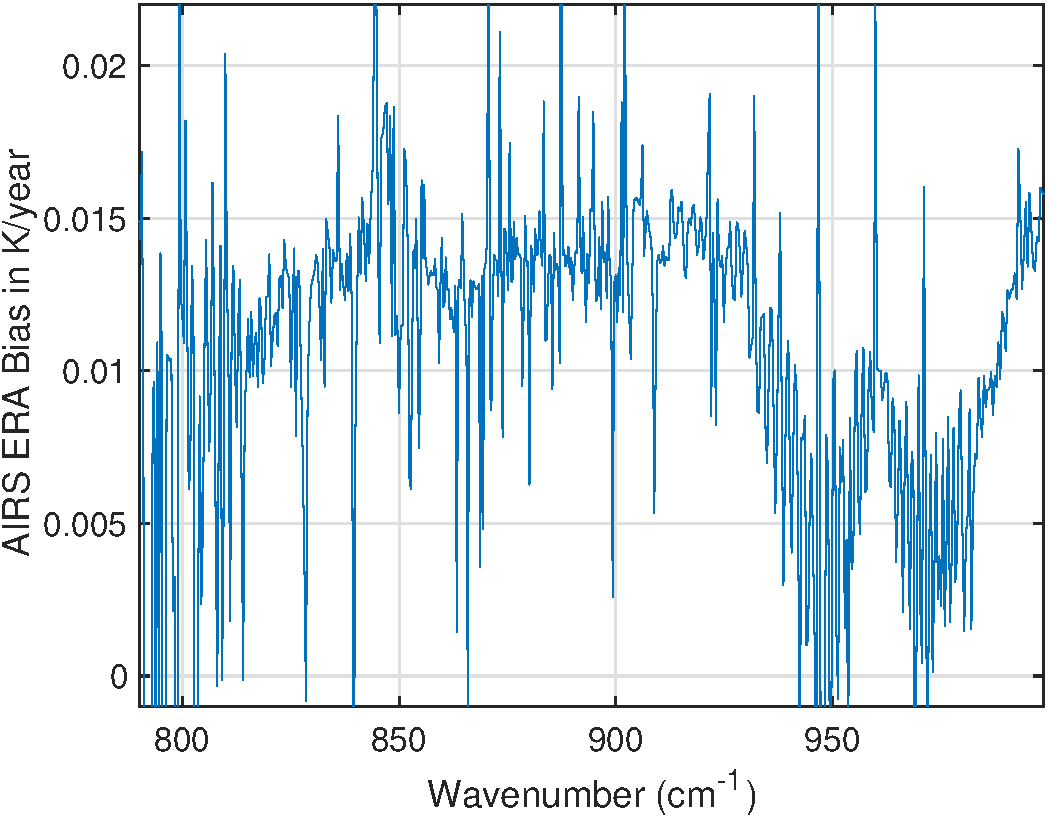
\includegraphics[width=0.75\linewidth]{./Figs/Pdf/airs_cfc_bias_iasi_times.pdf}
\end{center}
\end{block}
\end{column}
\end{columns}
\end{frame}

\begin{frame}[label={sec:org2d74f0d}]{Fit to AIRS CFC-11 for Removal in Fit Residuals}
\vspace{-0.3in}
\begin{columns}
\begin{column}{0.55\columnwidth}
\begin{block}{\footnotesize CFC-11 B(T) Trend}
\vspace{-0.1in}
\begin{center}
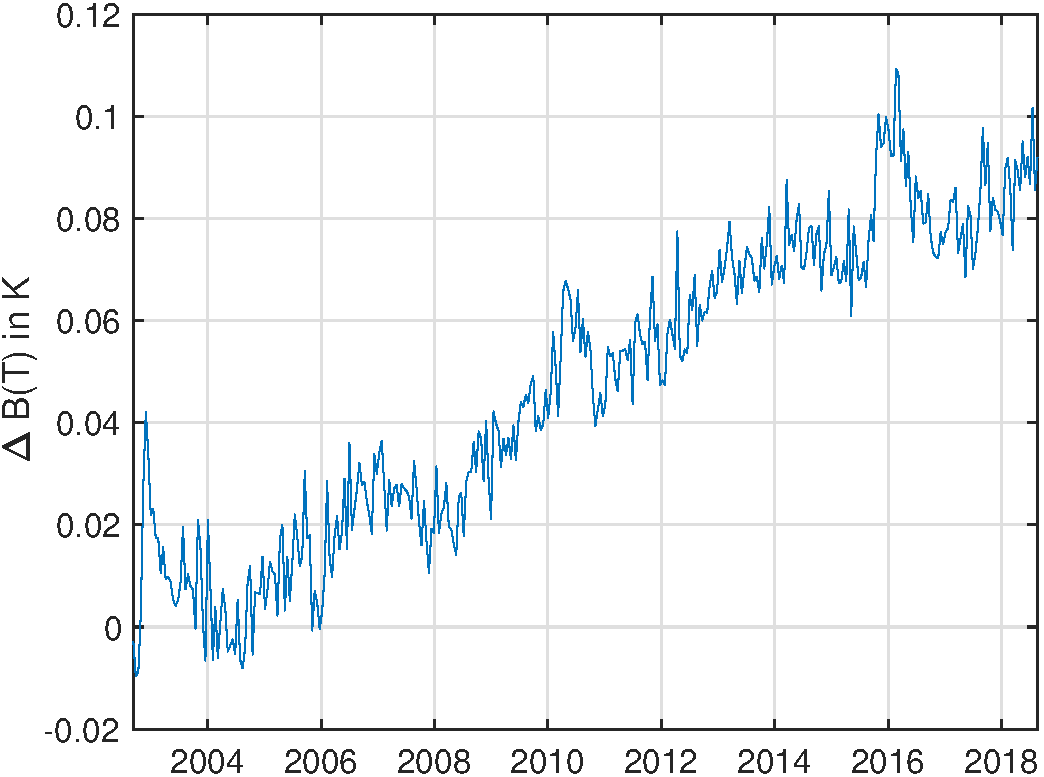
\includegraphics[width=0.85\linewidth]{./Figs/Pdf/cfc11_bt_trend.pdf}
\end{center}
\end{block}
\end{column}

\begin{column}{0.55\columnwidth}
\begin{block}{\footnotesize CFC ppb Trend}
\vspace{-0.1in}
\begin{center}
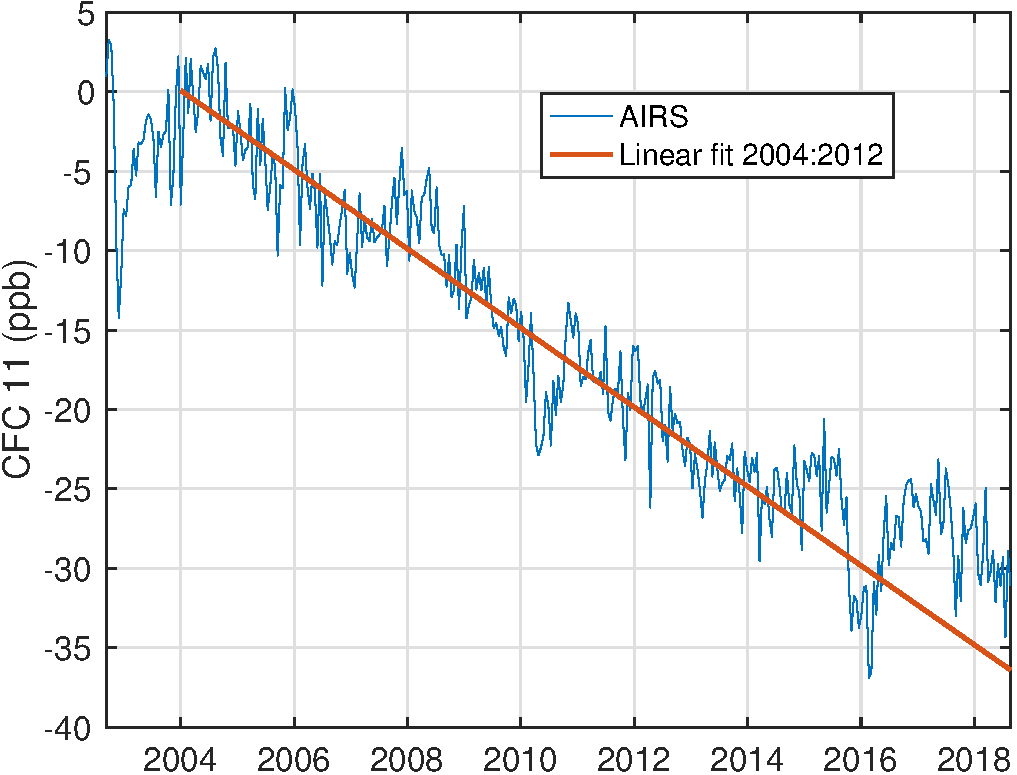
\includegraphics[width=0.85\linewidth]{./Figs/Pdf/cfc11_trend.pdf}
\end{center}
\end{block}
\end{column}
\end{columns}

\begin{footnotesize}
\begin{itemize}
\item Reasonably linear negative trend, as expected
\item Values agree well with in-situ
\item BUT, the trend appears to be decreasing!
\item Also expected from in-situ: possible cause is Chinese production of CFC-11
\item ENSO signals in time series: retrieval problem or something real?
\item Clear problems due to Nov. 2003 AQUA shutdown
\end{itemize}
\end{footnotesize}
\end{frame}
\begin{frame}[label={sec:org2874479}]{SST Retrieved from Anomaly Fits}
\vspace{-0.2in}
\begin{center}
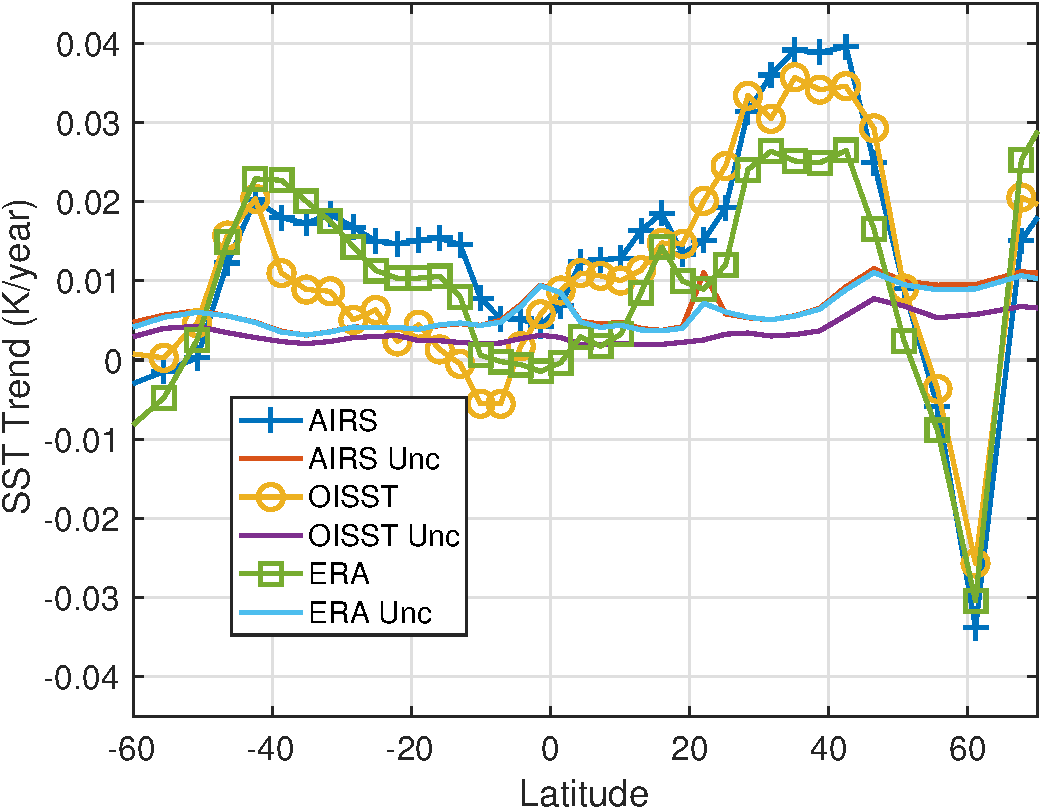
\includegraphics[width=0.7\linewidth]{./Figs/Pdf/co2_anom_sst_vs_oisst_clear_sampled_and_era.pdf}
\end{center}
\begin{footnotesize}
\begin{itemize}
\item OISST likely better?  AIRS-OISST = +0.005 \textpm{} 0.007 K/year (tropics)
\item ERA transitioned from RTG to OSTIA in Feb. 2009, we likely see that
\item Differences very small and at limits of SST climatologies
\end{itemize}
\end{footnotesize}
\end{frame}

\begin{frame}[label={sec:orgc28c0e9}]{Png/best\_co2\_anom\_resid.png}
\begin{center}
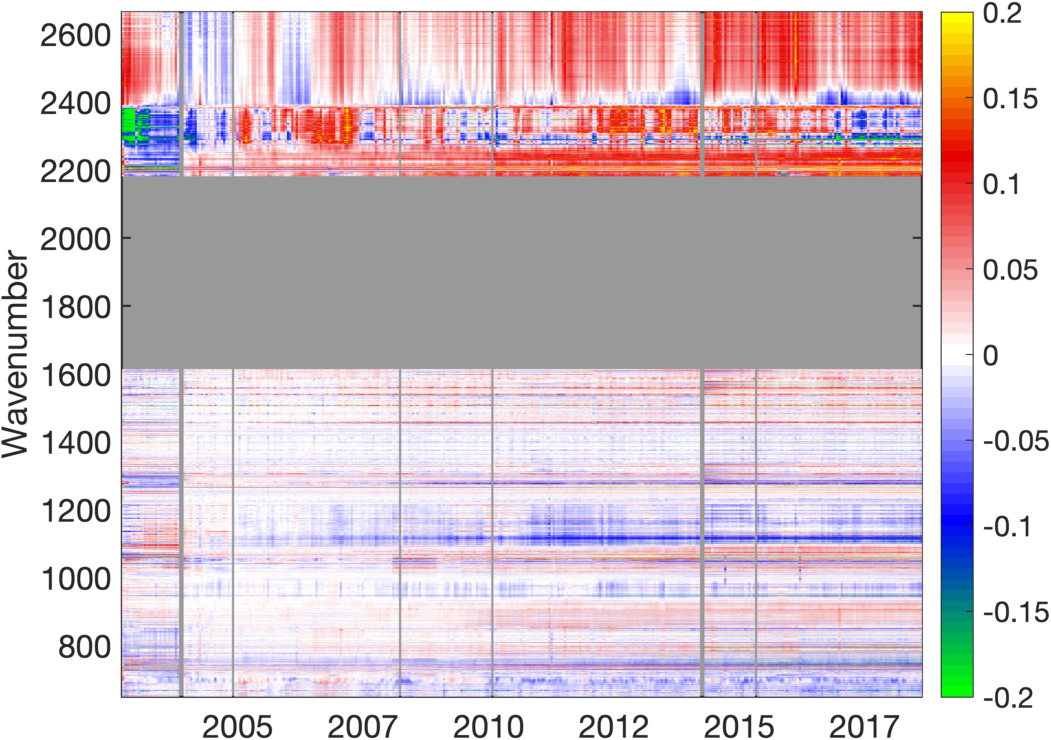
\includegraphics[width=0.7\linewidth]{./Figs/Png/best_co2_anom_resid.png}
\end{center}
\end{frame}

\begin{frame}[label={sec:org878893e}]{Png/best\_co2\_anom\_resid\_no\_sw.png}
\begin{center}
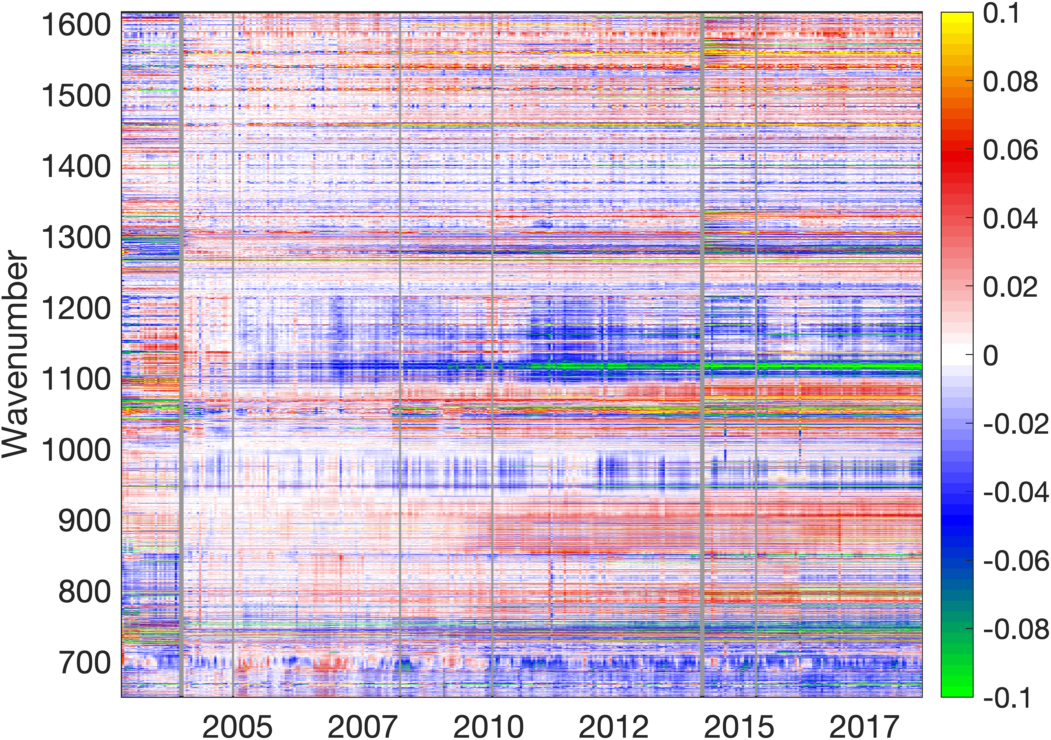
\includegraphics[width=0.7\linewidth]{./Figs/Png/best_co2_anom_resid_no_sw.png}
\end{center}
\end{frame}

\begin{frame}[label={sec:orgf4832a9}]{Png/best\_co2\_anomaly\_resid\_fit\_chans\_concat.png}
\begin{center}
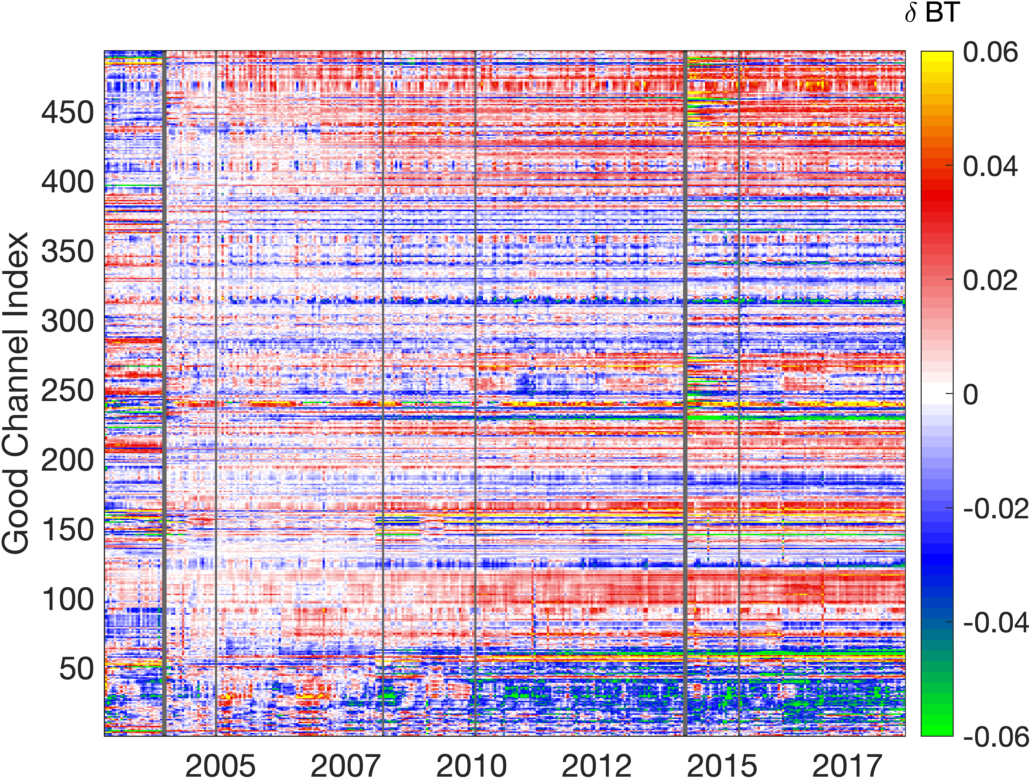
\includegraphics[width=0.7\linewidth]{./Figs/Png/best_co2_anomaly_resid_fit_chans_concat.png}
\end{center}
\end{frame}

\begin{frame}[label={sec:org7892f9f}]{Pdf/bt\_drift\_from\_anom\_resid\_2613\_chan.pdf}
\begin{columns}
\begin{column}{0.6\columnwidth}
\begin{block}{}
\vspace{-0.3in}
\begin{center}
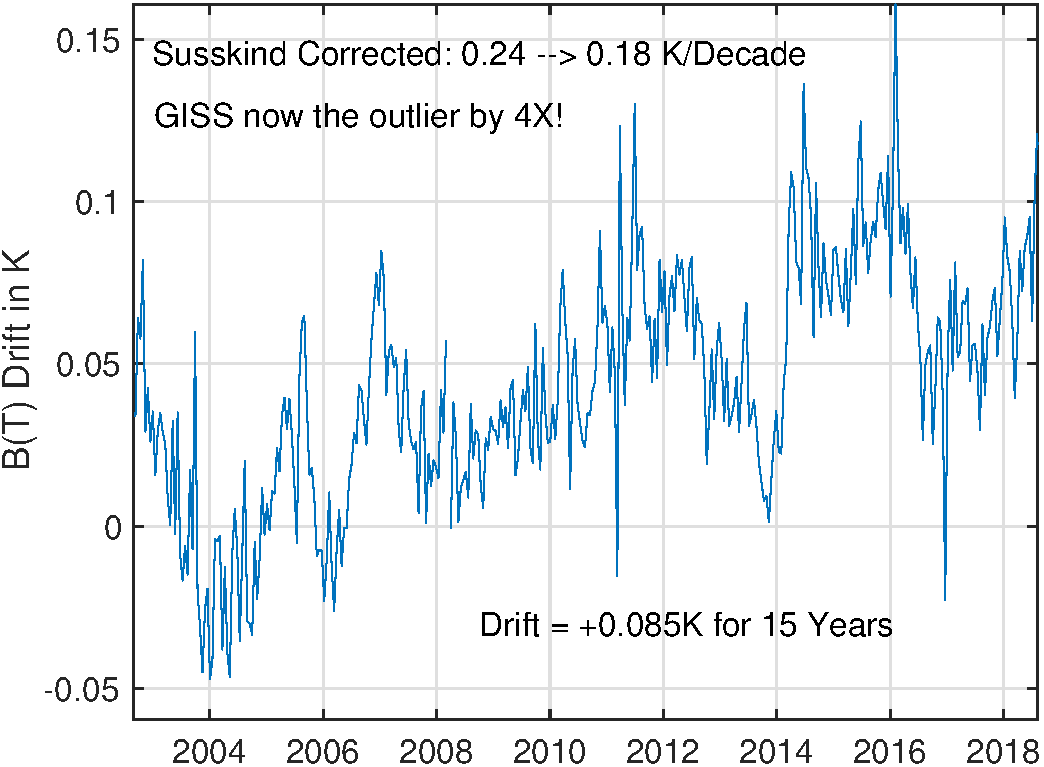
\includegraphics[width=\linewidth]{./Figs/Pdf/bt_drift_from_anom_resid_2613_chan_v2.pdf}
\end{center}
\end{block}
\end{column}

\begin{column}{0.4\columnwidth}
\begin{block}{From Susskind et. al.}
\begin{small}
\begin{center}
\begin{tabular}{ll}
AIRS & 0.24 \textpm{} 0.12\\
AIRS Corrected & 0.18\\
GISTEMP & 0.22 \textpm{} 0.13\\
HadCRUT4 & 0.17 \textpm{} 0.13\\
C\&W & 0.19 \textpm{} 0.12\\
ECMWF & 0.20 \textpm{} 0.16\\
UAH LT & 0.18\\
\end{tabular}
\end{center}
\end{small}
\end{block}
\end{column}
\end{columns}

Shortwave drift correction reduces AIRS global temperature trend by 33\% and bring AIRS into close agreement with HadCRUT4, C\&W, and UAH LT, signficantly worse agreement with GISTEMP.
\end{frame}

\begin{frame}[label={sec:orgf6abfb0}]{Latitude Dependence Surface Trends}
\vspace{-0.3in}
\begin{columns}
\begin{column}{0.55\columnwidth}
\begin{block}{Susskind 2019: SW}
\begin{center}
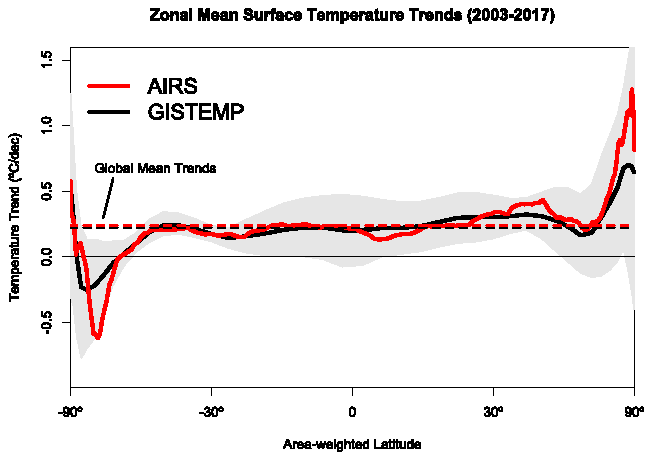
\includegraphics[width=\linewidth]{./Figs/Pdf/susskind_giss_trend_vs_lat.pdf}
\end{center}
\end{block}
\end{column}

\begin{column}{0.55\columnwidth}
\begin{block}{UMBC Trends: LW and SW}
\vspace{0.14in}
\begin{center}
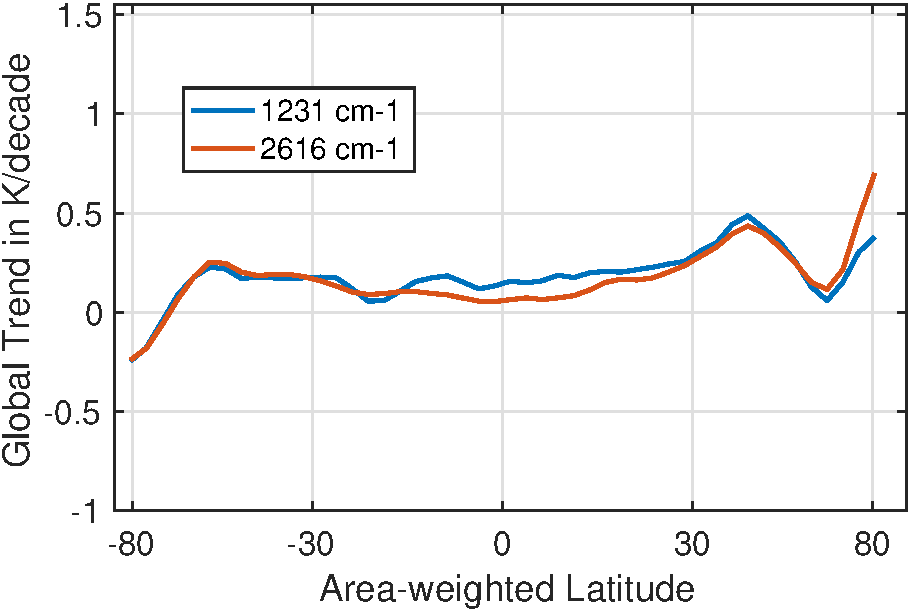
\includegraphics[width=\linewidth]{./Figs/Pdf/bt_global_trend_area_weight_lat_1231_vs_2616_from_hottest_v2.pdf}
\end{center}
\end{block}
\end{column}
\end{columns}

\vspace{-0.15in}
\begin{footnotesize}
Global Means
\begin{center}
\begin{tabular}{rrrrr}
GISS & Susskind & UMBC-1231 & UMBC-2616 & HadCRUT4\\
0.22 & 0.24 & 0.18 & 0.17 & 0.17\\
\end{tabular}
\end{center}

\vspace{-0.05in}
But, why isn't UMBC-2616 0.05K higher??\\
Note high/low Susskind values at poles not matched by UMBC\\
\emph{Rough} estimate for 2616 scene dependence: 0.06K/decade, Obs: 0.09K/decade\\
But what about the S. Pole??
\end{footnotesize}
\end{frame}

\begin{frame}[label={sec:org267b8e5}]{Pdf/resid\_spectrum\_dec17\_minus\_oct14\_2003.pdf}
\begin{center}
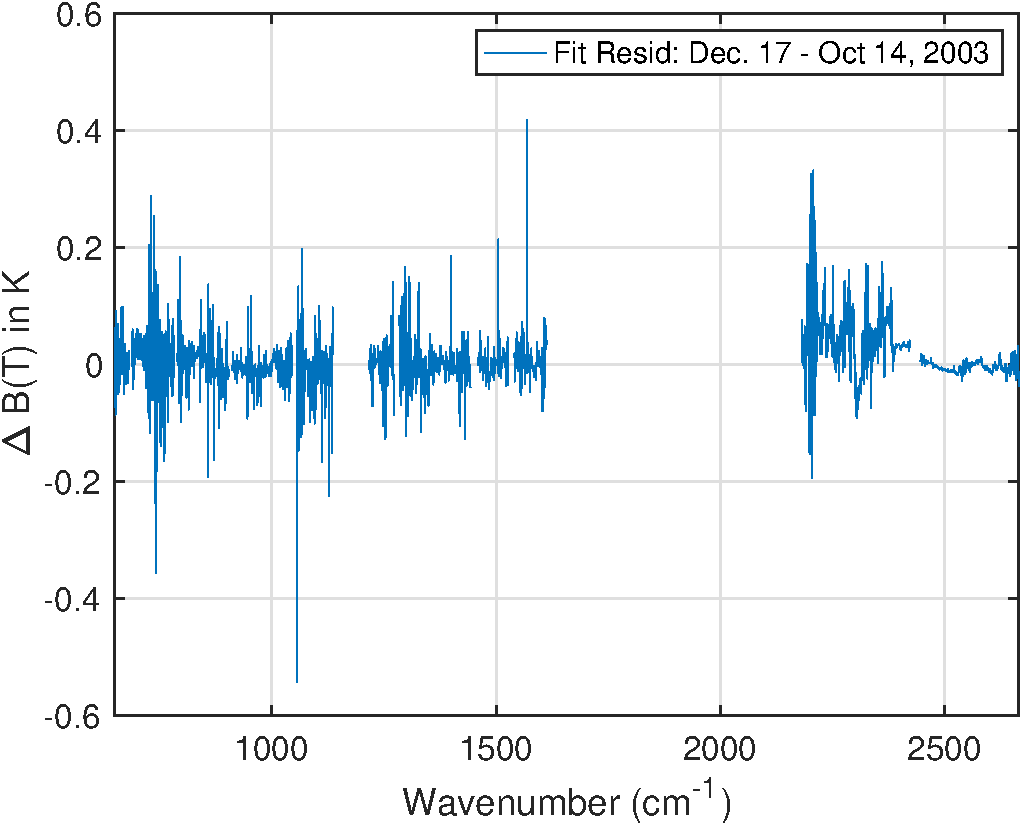
\includegraphics[width=0.7\linewidth]{./Figs/Pdf/resid_spectrum_dec17_minus_oct14_2003.pdf}
\end{center}
\end{frame}

\begin{frame}[label={sec:org25827b1}]{Pdf/resid\_spectrum\_dec17\_minus\_oct14\_2003\_swzoom.pdf}
\begin{center}
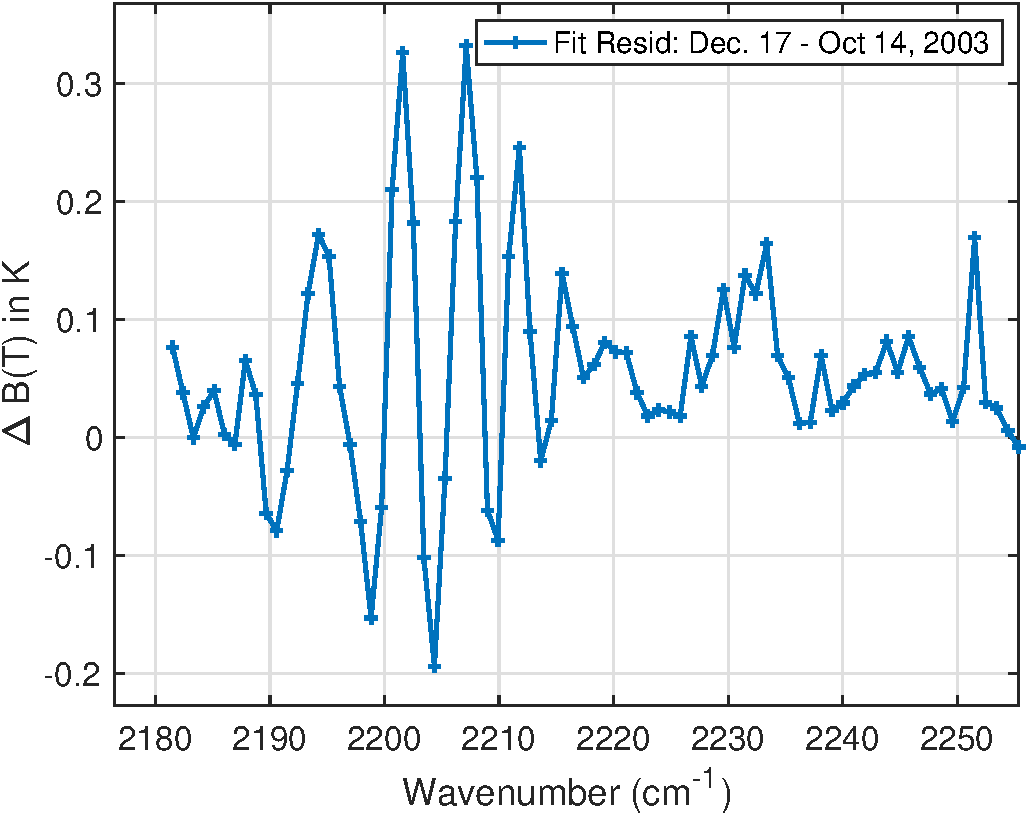
\includegraphics[width=0.7\linewidth]{./Figs/Pdf/resid_spectrum_dec17_minus_oct14_2003_swzoom.pdf}
\end{center}
\end{frame}

\begin{frame}[label={sec:orgeb69b0b}]{Pdf/resid\_1567\_and\_1570\_cm01\_dnu.pdf}
\begin{center}
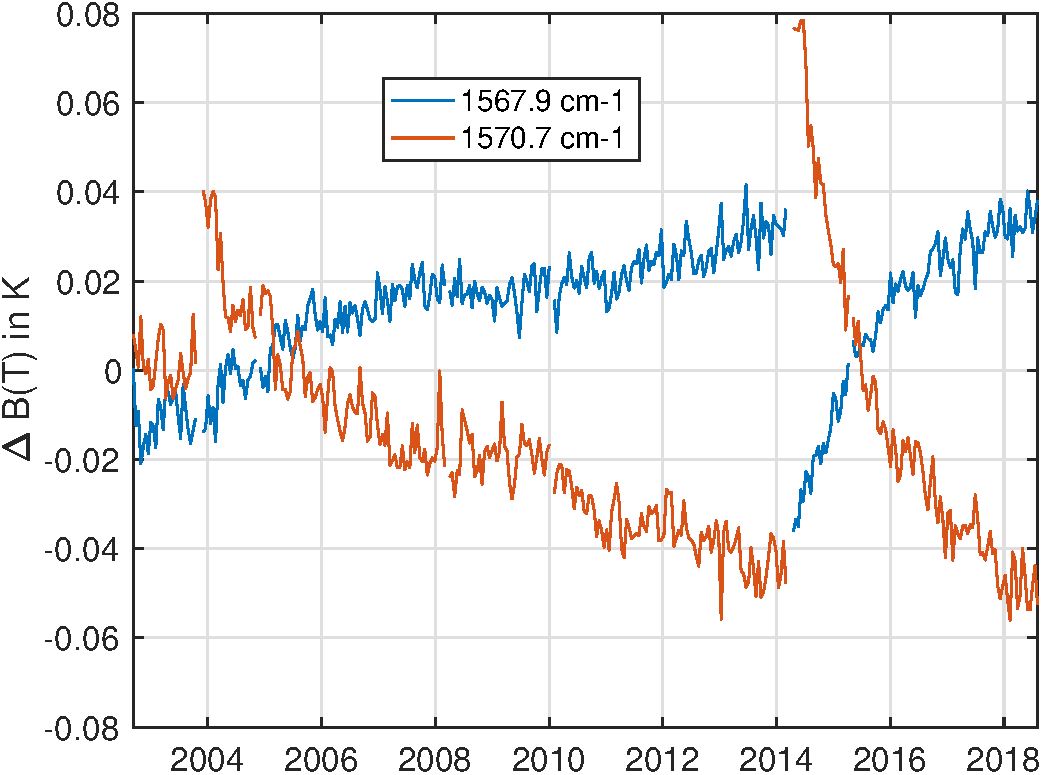
\includegraphics[width=0.7\linewidth]{./Figs/Pdf/resid_1567_and_1570_cm01_dnu.pdf}
\end{center}
\end{frame}

\begin{frame}[label={sec:org9dd777f}]{DCC1}
\begin{figure}[htbp]
\centering
\includegraphics[width=0.7\linewidth]{./Figsdc/Pdf/bt2616_and_bt960_dcc_vs_time_airs_and_iasi.pdf}
\caption{\emph{AIRS and IASI Dcc daily average temperatures versus time.  The IASI curve for 2616 cm\textsuperscript{-1} is an average over 54 IASI channels.}}
\end{figure}
\end{frame}

\begin{frame}[label={sec:org65d09f5}]{DCC4}
\begin{figure}[htbp]
\centering
\includegraphics[width=0.7\linewidth]{./Figsdc/Pdf/airs_iasi_dcc_rate_sw_iasi_avgpts.pdf}
\caption{\emph{Same as Fig. where? with every two points in IASI averaged.}}
\end{figure}
\end{frame}

\begin{frame}[label={sec:orge13b5dc}]{DCC6}
\begin{figure}[htbp]
\centering
\includegraphics[width=0.7\linewidth]{./Figsdc/Pdf/airs_iasi_dcc_rate_lw_ab_diffs_vs_iasi.pdf}
\caption{\emph{Longwave DCC linear rate of change with AIRS A,B, AB channels identifications highlighted.}}
\end{figure}
\end{frame}


\begin{frame}[label={sec:org9ad207c}]{overroye\_scan.pdf}
\begin{center}
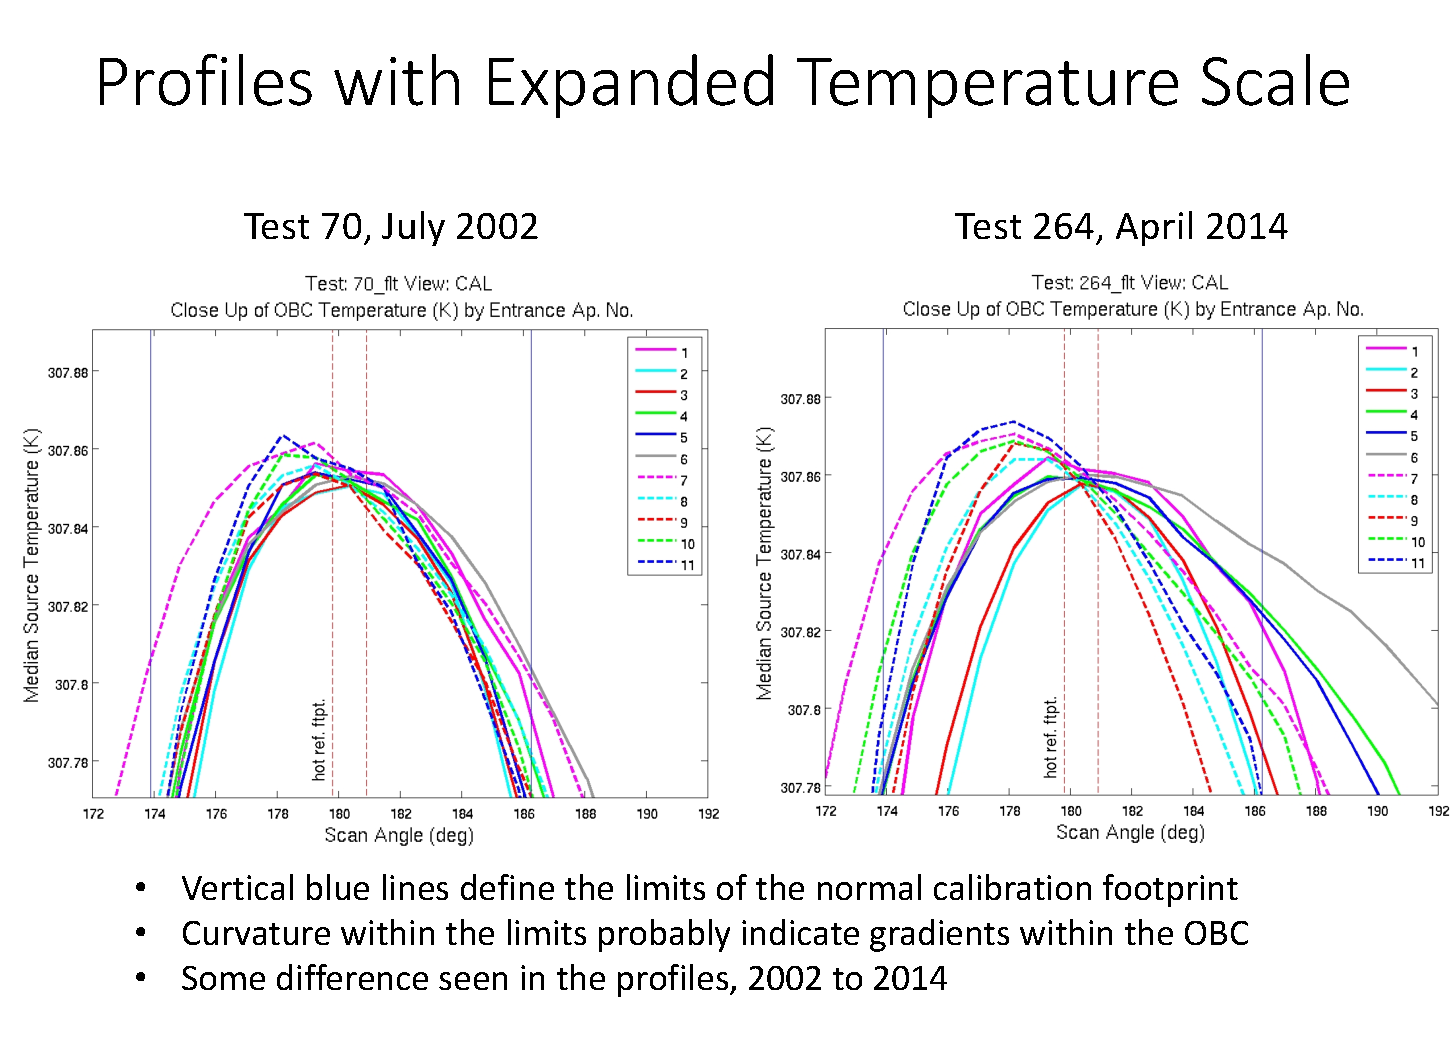
\includegraphics[width=0.7\linewidth]{./Figs/Pdf/overroye_scan.pdf}
\end{center}
\end{frame}

\begin{frame}[label={sec:orgbbf839e}]{overroye\_map.pdf}
\begin{center}
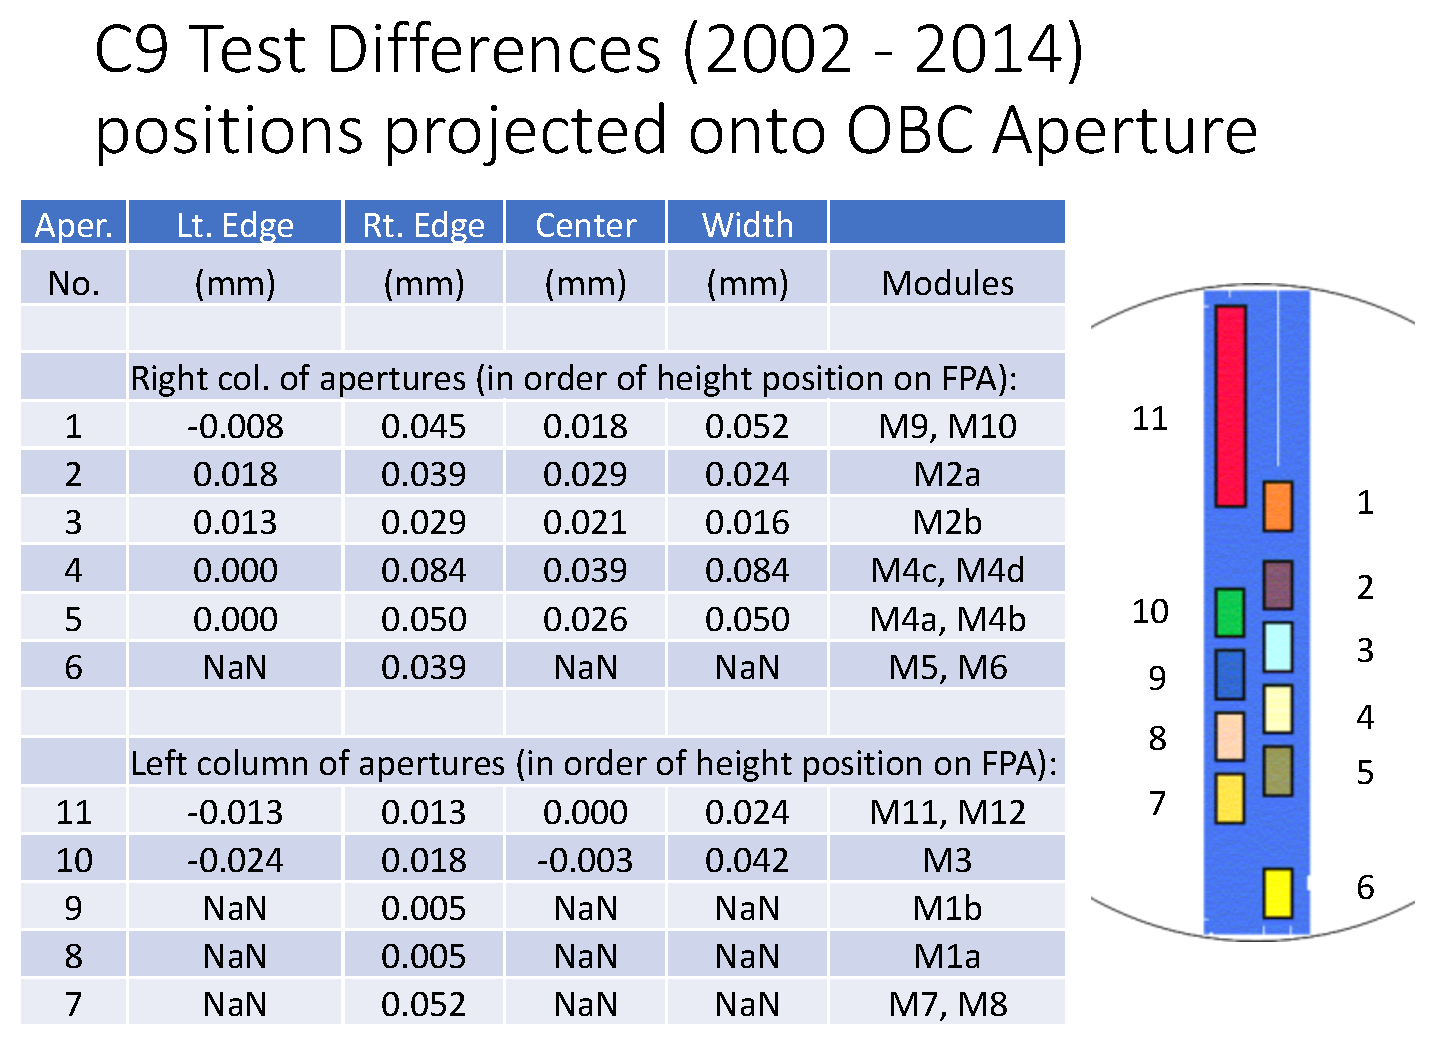
\includegraphics[width=0.7\linewidth]{./Figs/Pdf/overroye_map.pdf}
\end{center}
\end{frame}


\begin{frame}[label={sec:org7abc5e9}]{Surface T Trends Using 1231 \wn Channel}
\vspace{-0.35in}

\begin{columns}
\begin{column}{0.55\columnwidth}
\begin{block}{\footnotesize AIRS 1231 \wn}
\vspace{-0.1in}
\begin{center}
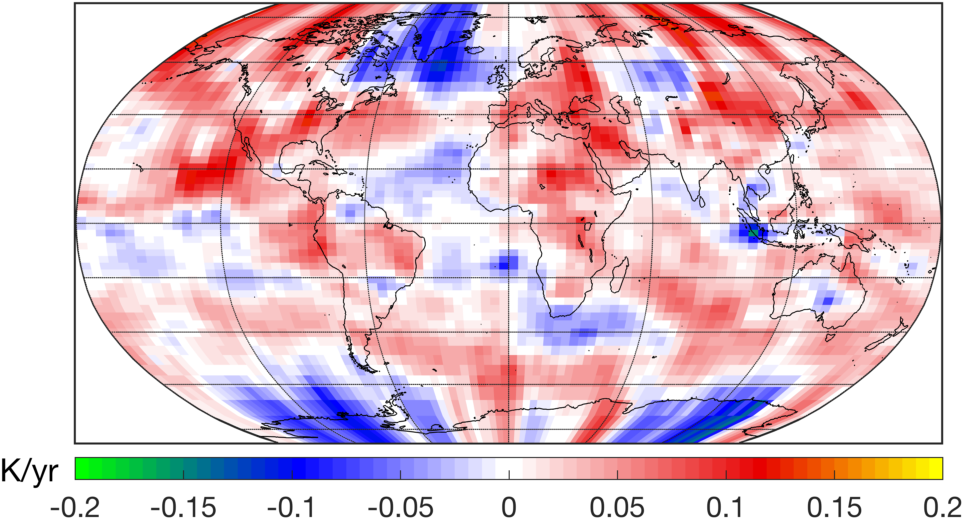
\includegraphics[width=\linewidth]{./Figs/Png/airs_tsurf_trend_from_1231cm_trend.png}
\end{center}
\end{block}
\end{column}

\begin{column}{0.55\columnwidth}
\begin{block}{\footnotesize ERA}
\vspace{-0.1in}
\begin{center}
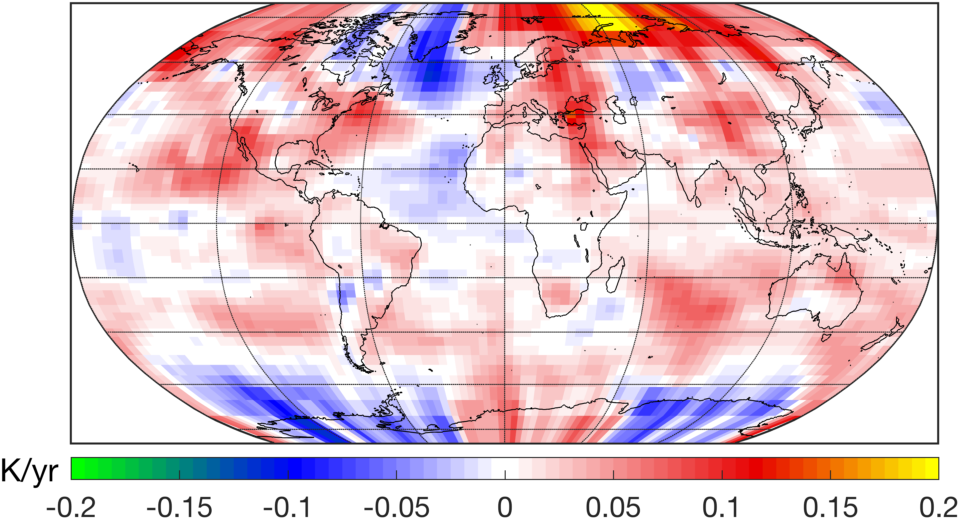
\includegraphics[width=\linewidth]{./Figs/Png/era_tsurf_trend.png}
\end{center}
\end{block}
\end{column}
\end{columns}


\begin{columns}
\begin{column}{0.55\columnwidth}
\begin{block}{\footnotesize OISST}
\vspace{-0.1in}
\begin{center}
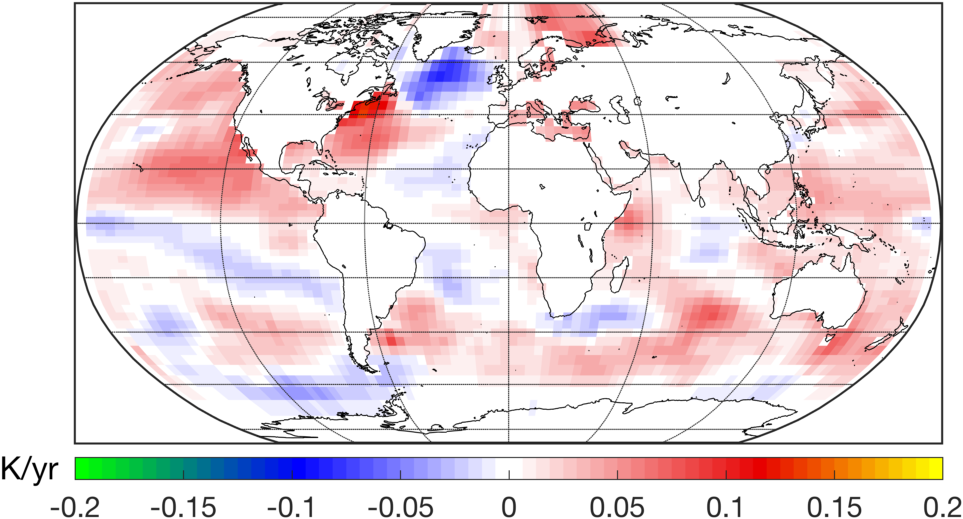
\includegraphics[width=\linewidth]{./Figs/Png/oisst_trend_map.png}
\end{center}
\end{block}
\end{column}

\begin{column}{0.5\columnwidth}
\begin{block}{\footnotesize AIRS 2616 \wn}
\vspace{-0.1in}
\begin{center}
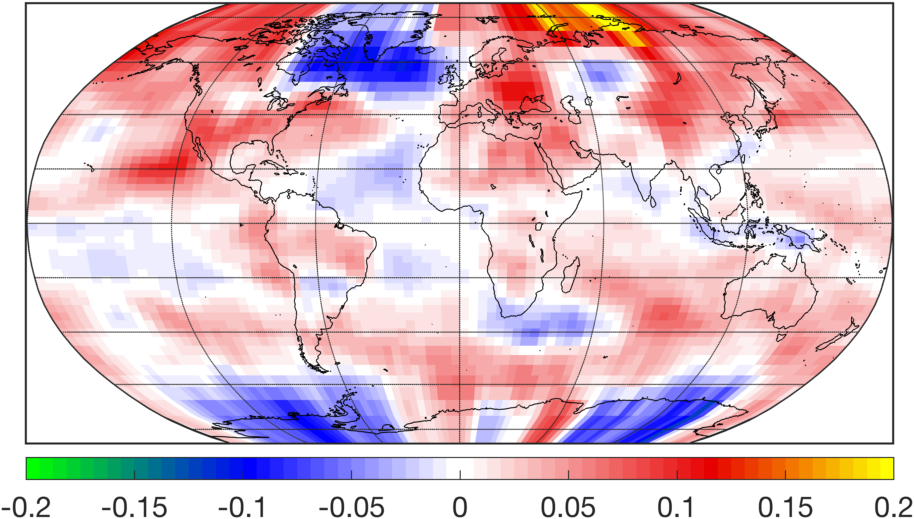
\includegraphics[width=\linewidth]{./Figs/Png/airs_tsurf_trend_from_2616cm_trend.png}
\end{center}
\end{block}
\end{column}
\end{columns}
\end{frame}


\begin{frame}[label={sec:org3a67ddb}]{Pdf/zonal\_sst\_trends\_12311\_vs\_oisst\_ersst5\_hottest\_per\_grid\_envelope.pdf}
\begin{center}
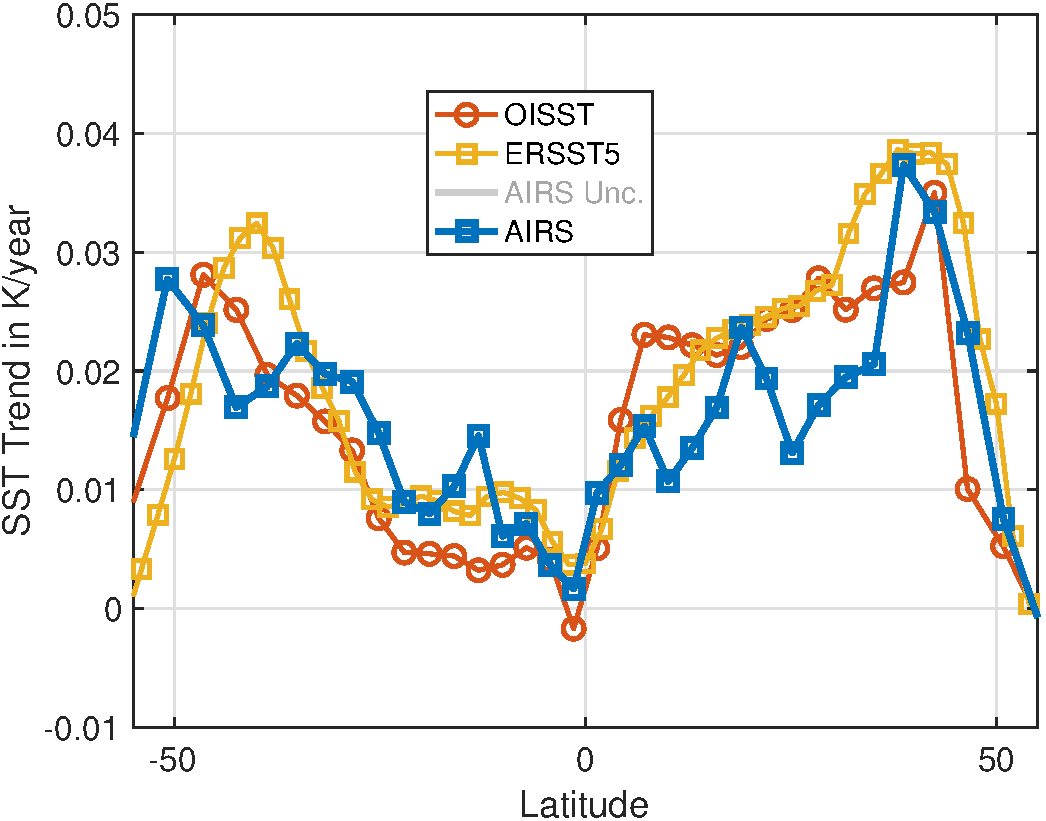
\includegraphics[width=0.7\linewidth]{./Figs/Pdf/zonal_sst_trends_12311_vs_oisst_ersst5_hottest_per_grid_envelope.pdf}
\end{center}
\end{frame}
\end{document}